\documentclass[a4paper,12pt]{report}
\usepackage{mypackage}

\title{Linear Algebra}

\author{Haydn Cheng}

\date{}

\begin{document}
\maketitle
\tableofcontents


\chapter{Vectors and Vector Spaces}

\section{Vectors in \(\mathbb{R}^{n}  \) }

Generally, a field \(F\)  (such as the set of all real numbers \(\mathbb{R}\) or complex numbers \(\mathbb{C}\)\footnote{More examples of fields are given in \cref{fields}.}) is an arena within which ``regular calculations'' involving addition and multiplication of numbers can be carried out. 

By \(F^{n} \) we denote the set of all ordered n-tuples of elements from field \(F\)

\begin{equation}
    F^{n} = \left\{ (a_1 , a_2 ,\ldots ,a_{n} ) \mid a_{i} \in F, i = 1,2,\ldots ,n  \right\}.
\end{equation}

As we will see, since \(F^{n} \) satisfies the definition of a vector space, so every n-tuple are already vectors themselves. However, we would usually arrange the elements of the n-tuples into the entries of a \(n\)-dimensional column vector as \(\vb{v} = \begin{pmatrix}
    a_1  & a_2  & \cdots  & a_{n}   \\
\end{pmatrix}^T\) for easier manipulation. 

It has a canonical (standard) basis, called the standard unit vectors, which are the \(n\) vectors in \(F^{n} \) where all the entries are zero excpet for the \(i^{\text{th }} \) element:  
\begin{equation}
    \vb{e} _{i} = (0,\ldots ,0,\underbrace{1}_{i^{\text{th }} \text{position} }, 0, \ldots , 0) = \begin{pmatrix}
         0 \\
         \vdots  \\
         0 \\
         1 \\
         0 \\
         \vdots  \\
         1 \\
    \end{pmatrix} \leftarrow i^{\text{th }} \text{position}.
\end{equation}

They are useful because a general vector in \(\mathbb{R} ^{n} \) can then be written as a linear combination of the unit vectors

\begin{equation}
    \vb{v} = v_{1} \vb{e} _{1} + \ldots + v_{n} \vb{e} _{n} = \sum_{i=1}^{n} v_{i} \vb{e} _{i} .  
\end{equation}

It is important to note that the concept of ``standard unit vectors'' is only appliacble to \(\mathbb{F}^{n} \). However, in later sections, we would introduce another concept (orthogonality) which extends this concept to any vector space.

  
\example{Google's search alogorithm}
{Consider an internet with \(n\) websites labeled by \(k = 1, \ldots , n\). The site labeled as \(k\) has been referenced to by other sites \(L_{k} \subset {1, \ldots , n}\). Assign a page rank to each website representing the relative significance of each website.}
{A first attempt would be to define the page rank as the number of pages that reference this page, so 

\begin{equation}
    x_{k} = n_{k}.
\end{equation}

An improved version would be to take into account the page rank of the pages that reference this page, as it is more desirable to be referenced by a page with higher page rank. So 

\begin{equation}
    x_{k} = \sum_{j \in L_{k} }^{} x_{j}   
\end{equation}

would be a improvement to the formula. Futhermore, as a reference is more valuable if a page only reference a samll number of page, we may define the page rank as 

\begin{equation}
    x_{k} = \sum_{j \in L_{k} }^{} \frac{x_{j} }{n_{j} }.   
\end{equation}

A simple example is illustrated below:

\begin{center}
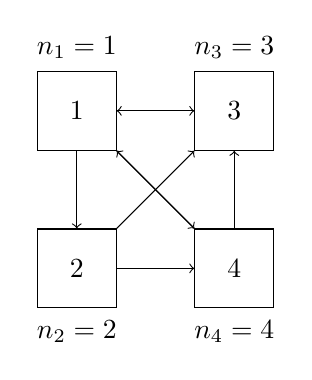
\begin{tikzpicture}
    % Node styles
    \tikzstyle{node_style} = [rectangle, draw, minimum size=1cm]
    
    % Nodes
    \node[node_style] (1) at (0,2) {1};
    \node[node_style] (2) at (0,0) {2};
    \node[node_style] (3) at (2,2) {3};
    \node[node_style] (4) at (2,0) {4};

    % Labels for n values
    \node at (0,2.8) {$n_1 = 1$};
    \node at (0,-0.8) {$n_2 = 2$};
    \node at (2,2.8) {$n_3 = 3$};
    \node at (2,-0.8) {$n_4 = 4$};

    % Arrows
    \draw[->] (1) -- (2);
    \draw[->] (1) -- (3);
    \draw[->] (2) -- (4);
    \draw[->] (4) -- (3);
    \draw[->] (4) -- (1);
    \draw[->] (2) -- (3);
    \draw[->] (3) -- (1);
    \draw[->] (1) -- (4);
\end{tikzpicture}
\end{center}

As shown in the figure, \(n=4, n_{1}=3, n_{2} = 2, n_3 = 1, n_4 = 2, L_{1} = {3,4}, L_{2} = {1}, L_3 = {1,2,4} \text { and } L_4 = {1,2}\). So the formulas for assigning the page rank becomes

\begin{equation}
    \begin{aligned}
        x_{1} &= \frac{x_3}{1} + \frac{x_4}{2} \\
        x_{2} &= \frac{x_{1}}{3} \\
        x_3 &= \frac{x_{1}}{3} + \frac{x_{2}}{2} + \frac{x_4}{2} \\
        x_4 &= \frac{x_{1}}{3} + \frac{x_{2}}{2}.        
    \end{aligned}
\end{equation}

This system of linear equations can be written in vector and matrix notation, as 

\begin{equation}
    A\vb{x} = \vb{x} ,
\end{equation}

where 

\begin{equation}
    \vb{x} = \begin{pmatrix}
         x_{1} \\
         x_{2} \\
         x_3 \\
         x_4  \\
    \end{pmatrix} \text { and } A = \begin{pmatrix}
        0 & 0 & 1 &  \frac{1}{2} \\
        \frac{1}{3} & 0 & 0 & 0  \\
        \frac{1}{3}  & \frac{1}{2}  & 0 & \frac{1}{2}   \\
        \frac{1}{3}  & \frac{1}{2}  & 0 & 0  \\
    \end{pmatrix}.
\end{equation}

This equation describes a so-called ``eigenvalue problem'', which we will discuss in a later stage.}

\section{Vector Spaces}

We start by defining a vector space and a sub vector space:

\begin{definition}[Definition of a Vector Space]
A vector space V over a field F is a set with two operations:

\begin{enumerate}
    \item vector addition: \((\vb{v}, \vb{w}) \mapsto \vb{v} + \vb{w} \in V \), where \(\vb{v} , \vb{w} \in V\).
    \item scalar multiplication: \((\alpha ,\vb{v}) \mapsto \alpha \vb{v} \in V\), where \(\alpha \in F \text { and } \vb{v} \in V\). 
\end{enumerate}

And for all \(\vb{u} ,\vb{v} ,\vb{w} \in V\) and all \(\alpha ,\beta \in F\), these operations have to satisfy the following rules:

\begin{enumerate}[label=(A\arabic*)]\label{vectorspace} 
    \item ``Associativity'': \((\vb{u} + \vb{v} ) + \vb{w}  = \vb{u}  + (\vb{v} + \vb{w} )\) .
    \item ``Neutral element'': There exists a ``zero vector'', \(\boldsymbol{0} \in V\) so that \(0 + \vb{v} = \vb{v} \)  .
    \item ``Inverse element'': There exists an inverse, \(-\vb{v} \) with \(\vb{v} + (-\vb{v} ) = 0\).
    \item ``Commutativity'': \(\vb{v} + \vb{w} = \vb{w} + \vb{v} \).
    \item \(\alpha (\vb{v} +\vb{w} ) = \alpha \vb{v} + \alpha \vb{w} \).
    \item \((\alpha +\beta )\vb{v} = \alpha \vb{v} + \beta \vb{w} \).
    \item \((\alpha \beta )\vb{v} = \alpha (\beta \vb{v} )\).
    \item \(1\cdot \vb{v} = \vb{v} \)      .
\end{enumerate}

The elements \(\vb{v} \in V\) are called ``vectors'', the elements \(\alpha \in F\) of the field are called ``scalars''.  
\end{definition}

\begin{definition}[Definition of a Sub Vector Space] \label{subvectorspace} 
A sub vector space \(W \subset V \) is a non-empty subset of a vector space \(V\) which is closed under vector addition and scalar multiplication, \ie\footnote{The rigorous proof of a sub vector space is a vector space itself is provided in \cref{subvectorvectorapp}.} 

\begin{enumerate}[label=(B\arabic*)]
    \item \(\vb{w} _{1} + \vb{w} _{2} \in W ~~~ \forall ~ \vb{w} _{1} , \vb{w} _{2} \in W\).
    \item \(\alpha \vb{w} \in W ~~~ \forall ~ \alpha \in \vb{F} \text { and } \vb{w} \in W\).     
\end{enumerate}
\end{definition}

\section{Span and Linear Independence}

\begin{definition}[Definition of Span]
    The span of \(k\) vectors \(\vb{v} _{1} , \ldots , \vb{v} _{k} \) in a vector space \(V\) over a field \(F\) is the set of all linear combinations of all those vectors
\end{definition}

\begin{equation}
    \text{Span} (\vb{v} _{1}, \ldots ,\vb{v} _{k}  ) \equiv  \left\{\sum_{i=1}^{k} \alpha _{i}\vb{v} _{i} \mid  \alpha _{i}\in F    \right\}.
\end{equation}

\begin{definition}[Definition of Linear Independence]
Let \(V\) be a vector space over \(F\) and \(\alpha _{1}, \ldots , \alpha _{k} \in  F  \) scalars. A set of vectors \(\vb{v} _{1}, \ldots , \vb{v} _{k} \in V\) is called linearly independent if 

\begin{equation}
    \sum_{i=1}^{} \alpha _{i} \vb{v} _{i} = \boldsymbol{0} \implies \alpha _{i} = 0 ~~~ \forall ~ i.      
\end{equation}

Otherwise, the vectors are called linearly dependent. 
\end{definition}

\begin{corollary}
The vectors \(\vb{v} _{1}, \ldots , \vb{v} _{k}  \) are linearly dependent \(\iff \) One vector \(\vb{v} _{i} \) can be written as a linear combination of the others. 
\end{corollary}

\begin{proof}
Assume the vectors \(\vb{v} _{1}, \ldots , \vb{v} _{k}  \) are linearly dependent so that the equation \(\sum_{k=1}^{k} \alpha _{i} \vb{v} _{i}  = 0\) has a solution with at least one \(\alpha _{i} \neq 0 \), then we can solve for \(\vb{v} _{i} \) to get

\begin{equation}
    \vb{v} _{i} = -\frac{1}{\alpha _{i} } \sum_{j \neq i}^{} \alpha _{j} \vb{v} _{j} ,    
\end{equation}

where we expressed \(\vb{v} _{i} \) as a linear combination of the other vectors.

\end{proof}


\example{Linear Independence of Vectors in \(\mathbb{R}^3 \) }
{Verify the following vectors in \(\mathbb{R}^3 \) are linearly independent 

\begin{equation}
    \vb{v} _{1} = \begin{pmatrix}
         0 \\
         1 \\
         1 \\
    \end{pmatrix}, \vb{v} _{2} = \begin{pmatrix}
         0 \\
         1 \\
         2 \\
    \end{pmatrix}, \vb{v} _{3} = \begin{pmatrix}
         1 \\
         1 \\
         -1 \\
    \end{pmatrix}, 
\end{equation}}
{Setting the linear combination of vectors to be the zero vector,

\begin{equation}
    \alpha _{1}\vb{v} _{1} + \alpha _{2} \vb{v} _{2} + \alpha _{3} \vb{v} _{3} = \begin{pmatrix}
         \alpha _{3}  \\
         \alpha _{1} + \alpha _{2} + \alpha _{3}   \\
         \alpha _{1} + 2\alpha _{2} - \alpha _{3}   \\
    \end{pmatrix} = \boldsymbol{0} 
\end{equation}

we find that it only has the solution \((\alpha _{1}, \alpha _{2}, \alpha _{3}   ) = (0,0,0)\). Therefore the vectors are linearly independent.
} 

\example{Linear Independence of Solutions to Differential Equations}
{Prove that the solutions \(y(x) = \cos x \text { and } y(x) = \sin x\)  to the homogeneous, linear second order differential equation 

\begin{equation}
    \frac{d^2y}{dx^2} = -y
\end{equation}

are linearly indpendent.}
{We start with setting the linear combination of the solutions to 0,

\begin{equation}
    \alpha \sin x+ \beta \cos x= 0,
\end{equation}

and since the equation has to be satisfied for all \(x\),  setting \(x=0\) we learn that \(\beta =0\) and setting \(x=\frac{\pi }{2} \) it follows that \(\alpha = 0\). Hence \(\sin x\) and \(\cos x\)  are linearly independent. 
} 

\section{Basis and Dimension}
\begin{definition}[Definition of a Basis]
A set \(\vb{v} _{1}, \ldots , \vb{v} _{n} \in V \) of vectors is called a basis of \(V\) if and only if 

\begin{enumerate}[label=(C\arabic*)] \label{basis} 
    \item \(\vb{v} _{1}, \ldots , \vb{v} _{n}  \) are linearly independent.
    \item \(V = \text{Span}(\vb{v} _{1}, \ldots , \vb{v} _{n}  ) \)  
\end{enumerate}
\end{definition}

\begin{lemma} \label{uniquelinear} 
If \(\vb{v} _{1}, \ldots ,\vb{v} _{n}  \) is a basis of \(V\), every vector \(\vb{v} \in V\) can be written as a unique linear combination as

\begin{equation}
    \vb{v} = \sum_{i=1}^{n} \alpha _{i} \vb{v} _{i}  .
\end{equation}

\end{lemma}

\begin{proof}
Firstly we must be able to write \(\vb{v} \) as a linear combination of the basis, since \(\vb{v} \in V \text { and } V = \text{Span} (\vb{v}_1, \cdots, \vb{v}_n ) \).   

Now assume that \(\vb{v} \) can be written as two different linear combinations of the basis, \ie 

\begin{equation}
    \vb{v} = \sum_{i=1}^{n} \alpha _{i}\vb{v} _{i} = \sum_{i=1}^{n} \beta _{i} \vb{v} _{i}.  
\end{equation}

Taking the difference of these two equations implies

\begin{equation}
    \sum_{i=1}^{n} (\alpha _{i} - \beta _{i}  )\vb{v} _{i} =0
\end{equation}

and from linear independence of the basis, it follows that all \(\alpha _{i} - \beta _{i} = 0  \), so that indeed \(\alpha _{i} = \beta _{i}  \). 
\end{proof}

We would like to call the number of vectors in a basis the dimension of the vector space. First, however, we have to proof that the number of vectors in a basis of a vector space is an invariant.

\begin{lemma}[Exchange Lemma] \label{exchangelemma} 
Let \(\vb{v} _{1}, \ldots , \vb{v} _{n}  \) be a basis of \(V\) and \(\vb{w} _{1}, \ldots ,\vb{w} _{m} \in V \) arbitrary vectors. If \(m > n\) then \(\vb{w} _{1}, \ldots ,\vb{w} _{m}  \) are linearly dependent.  
\end{lemma}

\begin{proof}
Consider the first arbitrary vector \(\vb{w} _{1} \). If \(\vb{w} _{1} = 0 \) then the vectors \(\vb{w} _{1}, \ldots ,\vb{w} _{m}  \) are linearly dependent (since the coefficient of \(\vb{w} _{1} \) can be any arbirary constant when we write down the linaer combination of the vectors \(\vb{w}_1, \cdots, \vb{w}_n \) to test their linear dependency), so we can assume that \(\vb{w} _{1} \neq 0 \).    

Since the vectors \(\vb{v} _{i} \) form a basis we can write the first arbitrary vector as

\begin{equation}
    \vb{w} _{1} = \sum_{i=1}^{n} \alpha _{i} \vb{v} _{i}   
\end{equation}

with at least one \(\alpha _{i}\)  (say \(\alpha _{1} \)) non-zero (or else \(\vb{w} _{1} \) would be zero). We can therefore solve this equation for \(\vb{v} _{1} \) as

\begin{equation}
    \vb{v} _{1} = \frac{1}{\alpha _{1} } \left( \vb{w} _{1} - \sum_{i=2}^{n} \alpha _{i} \vb{v} _{i}   \right). \label{exchangev1} 
\end{equation}

This shows that we use \(\vb{w} _{1} \) to replace \(\vb{v} _{1} \) in basis \(\vb{v}_{1}, \ldots, \vb{v}_n \) such that \(V = \text{Span}(\vb{w} _{1}, \vb{v}_{2}, \ldots, \vb{v}_n  ) \), such that the span is remained unchanged. This is because any vector \(\vb{u} \in V\) which can be written as a linear combination of the basis \(\vb{v}_{1}, \ldots, \vb{v}_n \) can now be written as a linear combination of the basis \(\vb{w} _{1}, \vb{v}_{2}, \ldots, \vb{v}_n \) simply by utilizing \cref{exchangev1}.     

This exchange process can be repeated until all \(\vb{v} _{i} \) are placed by \(\vb{w} _{i} \) and \(V = \text{Span} (\vb{w}_{1}, \ldots, \vb{w}_n ) \). Since \(m > n\) there is at least one vector \(\vb{w} _{n+1} \) ``left over'' which can be written as a lniear combination 

\begin{equation}
    \vb{w} _{n+1} = \sum_{i=1}^{n} \beta _{i} \vb{w} _{i}  
\end{equation}

which shows that the vectors \(\vb{w}_{1}, \ldots, \vb{w}_m\) are linearly dependent.
\end{proof}

\begin{definition}[Definition of Dimension] \label{dimension} 
For a basis \(\vb{v}_{1}, \ldots, \vb{v}_n \) of a vector space \(V\) over \(F\) we call \(\dim _{F} (V) \equiv n \) the dimension of \(V\) over \(F\) . 
\end{definition}

\example{Standard Unit Vectors form a Basis}
{Prove that the standard unit vectors \(\vb{e}_1, \cdots, \vb{e}_n \) form a basis over the vector space \(\mathbb{R}^{n} \text { and } \mathbb{C}^{n} \). }
{Set the linear combination of the standard unit vectors to zero, 

\begin{equation}
    \sum_{i=1}^{n} \alpha _{i} \vb{e} _{i} = \begin{pmatrix}
         \alpha _{1}  \\
         \vdots  \\
         \alpha _{n}  \\
    \end{pmatrix} =0
\end{equation}

which is only true if \(\alpha _{i} = 0 ~ \forall ~ i\).

Thus the standard unit vectors \(\vb{e}_{1}, \ldots, \vb{e}_n \) form a basis of \(\mathbb{R}^{n} \text { and } \mathbb{C}^{n}  \) seen as vector spaces of the fields \(\mathbb{R}\text { and } \mathbb{C}\), respectively, where the dimensions are 

\begin{equation}
    \dim _{\mathbb{R}} (\mathbb{R}^{n} ) = \dim _{\mathbb{C}} (\mathbb{C}^{n} ) = n. 
\end{equation}

However, note that \(\mathbb{C}^{n} \) as a vector space over \(\mathbb{R}\) has a basis \(\vb{e}_{1}, \ldots, \vb{e}_n, i \vb{e} _{1}, \ldots , i \vb{e} _{n}   \) and therefore \(\dim _{\mathbb{R}} (\mathbb{C}^{n} ) = 2n\). 
} 

\example{Basis of a Polynomial}
{Prove that the monomials \(1,x,^2,\ldots ,x^{d} \) form a basis over a vector space containing all real polynomials of degree \(d\).}
{We start with setting  
\begin{equation}
    \sum_{i=0}^{d} \alpha _{i} \vb{x} ^{i} =0 
\end{equation}

to check if there is any non-trivial solution. However, by taking the \(k^{\text{th }} \)derivative with respect to \(x\) and then set \(x=0\) (since it has to satisfy for all \(x\)), this immediately implies that \(\alpha _{k} = 0 ~ \forall ~  k\) and hence the monomials are linearly independent and form a basis and the vector space has dimension \(d+1\).
}

\example{Basis of a \(n \times m\) matrix }
{Find a basis and the dimension of the vector space containing all \(n \times m\) matrices with real entries.}
{The analogy of standard unit vectors for matrices is

\begin{equation} \label{matricesbasis} 
    E_{(ij)}  = \begin{pmatrix}
        0 & \ldots  & 0 & 0 & 0 & \ldots  &  0 \\
        \vdots  &  & \vdots  & \vdots  & \vdots  &  &  \vdots  \\
        0 & \ldots  & 0 & 0 & 0 & \ldots  &  0 \\
        0 & \ldots  & 0 & 1 & 0 & \ldots  &  0 \\
        0 & \ldots  & 0 & 0 & 0 & \ldots  &  0 \\
        \vdots  &  & \vdots  & \vdots  & \vdots  &  &  \vdots  \\
        0 & \ldots  & 0 & 0 & 0 & \ldots  &  0 \\
    \end{pmatrix}\footnote{Here the subscript \((i,j)\) has been used to indicate the row and column which have been changed rather than specific entries of the matrix. } 
\end{equation}

where \(i=1,\ldots ,n \text { and } j= 1,\ldots ,m\) and the ``1'' appears in the \(i^{\text{th }} \)row and the \(j^{\text{th }} \)column with all other entries zero. Clearly these matrices form a basis, in complete analogy with the standard unit vectors. Therefore the vector space of \(n\times m\) matrices has dimension \(nm\).    
} 

\begin{lemma}[Properties of a Vector Space]
For a vector sapce \(V\) spanned by a finite number of vectors we have:

\begin{enumerate}[label=(D\arabic*)] 
    \item \(V \) has a basis.
    \item Every linearly independent set \(\vb{v}_{1}, \ldots, \vb{v}_k \in V\) that is not already a basis of \(V\) can be completed by some other vectors in \(V\) to form a basis.
    \item If \(n = \dim (V)\), any linaerly independent set of vectors \(\vb{v}_{1}, \ldots, \vb{v}_n \) forms a basis.
    \item If \(\dim _{F} (V) = \dim _{F} (W)\) and \(V \subset W\) for two vector spaces \(V,W\) then \(V=W\).      
\end{enumerate}

\end{lemma}

\begin{proof}

\begin{enumerate}[label=(D\arabic*)] 
    \item Since \(V = \text{Span}(\vb{v}_{1}, \ldots, \vb{v}_k ) \), If these vectors are linearly independent we have found a basis. If not, one of the vectors, say \(v_{k} \) can be written as a linear combination of the others and can, hence, be dropped without changing the spoan, so \(V = \text{Span}(\vb{v}_{1}, \ldots, \vb{v}_{k-1}) \). This process can be continued until the remainng set of vectors is linaerly independent.
    \item If \(V= \text{Span}(\vb{v}_{1}, \ldots, \vb{v}_k) \) we are finished. If not there exists a vector \(\vb{v} _{k+1} \notin Span(\vb{v}_{1}, \ldots, \vb{v}_k) \). Hence the vectors \(\vb{v}_{1}, \ldots, \vb{v}_k, \vb{v} _{k+1} \) must be linaerly independent. We can continue adding vectors to the list until it spans the whole space. This process must terminate after a finite number of steps or else we would contradict the exchange \cref{exchangelemma}, which states that the number of vectors in a basis is an invariant.
    \item If \(\dim (V) = n\) and the linearly independent set \(\vb{v}_{1}, \ldots, \vb{v}_n \) did not span \(V\) then from (D2) it could be completed to a basis with more than \(n\) elements. However this is a contradiction since according to the exchange \cref{exchangelemma} the number of vectors in a basis is an invariant. So the vectors \(\vb{v}_{1}, \ldots, \vb{v}_n \) must span the space and they form a basis.
    \item We can choose a basis \(\vb{v}_{1}, \ldots, \vb{v}_n \) of V. Since \(V \subset W\), these basis vectors are linaerly independent in \(W\), and since \(\dim _{F} (W) = \dim _{F} (V)  \), they must also form a basis of \(W\), using (D3). Hence \(V = \text{Span}(\vb{v}_{1}, \ldots, \vb{v}_n ) = W \).         
\end{enumerate}

\end{proof}

\todo{magic square} 

\chapter{Vectors in \(\mathbb{R}^{n} \) and its Geometrical Applications }

\section{Scalar Product in \(\mathbb{R}^{n} \) }

The scalar (dot) product for two n-demensional column vectors is defined as

\begin{equation}
    \vb{a} \cdot \vb{b} \equiv \sum_{i=1}^{n} a_{i} b_{i} .
\end{equation}

In Einstein summation convention we simply write \(\vb{a} \cdot \vb{b} = a_{i} b_{i} \), assuming we sum over any index which appears twice in a given term.

The dot product satisfies a number of obvious properties, namely

\begin{enumerate}
    \item \(\vb{a} \cdot \vb{b} = a_{i} b_{i} = b_{i} a_{i} = \vb{b} \cdot \vb{a}  \)
    \item \(\vb{a} \cdot (\vb{b} + \vb{c} ) = a_{i} (b_{i} + c_{i}  ) = a_{i}b_{i} + a_{i}c_{i}   = \vb{a} \cdot \vb{b} + \vb{a} \cdot \vb{c}  \)
    \item \(\vb{a} \cdot (\beta \vb{b} ) = a_{i}(\beta b_{i} ) = \beta a_{i}b_{i} = \beta \vb{a} \cdot \vb{b}    \)
    \item \(\vb{a} \cdot \vb{a}  = \sum_{i=1}^{n} a_{i}^2 > 0 \text{for} \vb{a} \neq \boldsymbol{0}  \)
\end{enumerate}

The last property allows us to define the length of a vector as 

\begin{equation}
    \abs{\vb{a} } \equiv \sqrt{\vb{a} \cdot \vb{a} } = \left( \sum_{i=1}^{n} a_{i}^2  \right) ^{\frac{1}{2} }.   
\end{equation}

The dot product satisfies an important inequality 

\begin{lemma}[Cauchy-Schwarz inequality]
For any two vectors \(\vb{a} \) and \(\vb{b} \) in \(\mathbb{R}^{n} \) we have

\begin{equation}
    \abs{\vb{a} \cdot \vb{b} } \le \abs{\vb{a} }\abs{\vb{b} }.  
\end{equation}

\end{lemma}

\begin{proof}
Without loss of generality let \(\abs{\vb{a} } = \abs{\vb{b} } = 1  \) (if this is not the case then we can always normalize the vectors). Then

\begin{equation}
    0 \le \abs{\vb{a} \pm \vb{b} }^2 = (\vb{a} \pm \vb{b} )\cdot (\vb{a} \pm \vb{b} ) = \abs{\vb{a} }^2 + 2(\vb{a} \cdot \vb{b} ) + \abs{\vb{b} }^2 = 2(1 \pm \vb{a} \cdot \vb{b} ) \implies \abs{\vb{a} \cdot \vb{b} } \le 1. 
\end{equation}
\end{proof}

A closely related inequality is the famous

\begin{lemma}[Triangle Inequality]
For any two vectors \(\vb{a} \text { and } \vb{b} \) in \(\mathbb{R}^{n} \) we have

\begin{equation}
    \abs{\vb{a} + \vb{b} } \le \abs{\vb{a} } + \abs{\vb{b} }   
\end{equation}
\end{lemma}

\begin{proof}
\(\abs{\vb{a} +\vb{b} }^2 = \abs{\vb{a} }^2 + \abs{\vb{b} }^2 + 2 \vb{a} \cdot \vb{b} \le \abs{\vb{a} }^2 + \abs{\vb{b} }^2 + 2\abs{\vb{a} }\abs{\vb{b} } = (\abs{\vb{a} } + \abs{\vb{b} }  )^2      \). 
\end{proof}

For two non-zero vectors \(\vb{a} \text { and } \vb{b} \), the Cauchy-Schwarz inequality implies that we can define an unique angle \(\theta \in [0,\pi ]\) as

\begin{equation}
    -1 \le \cos \theta = \frac{\vb{a} \cdot \vb{b} }{\abs{a}\abs{b}  } \le 1 \implies \vb{a} \cdot \vb{b} = \abs{\vb{a} } \abs{\vb{b} }\cos \theta .  
\end{equation}

We call two vectors orthogonal (or perpendicular) if and only if \(\vb{a} \cdot \vb{b} = 0, \text { or }  \theta = \frac{\pi }{2} \).

\section{Vector Product in \(\mathbb{R}^3 \) }

\subsection{Triple Products}
	
\subsubsection{Scalar Triple Product \(\vb{A} \cdot (\vb{B} \cross \vb{C})\)}
	
The scalar triple product \(\vb{A} \cdot (\vb{B} \cross \vb{C})\) represents the volume of the parallelepiped generated by \(\vb{A}\), \(\vb{B}\) and \(\vb{C}\) (as shown in \cref{para}) since \(\abs{\vb{B} \cross \vb{C}}\) is the base area, and \(\abs{\vb{A}\cos{\theta}}\) is the altitude. Therefore, by considering different pairs of bases and altitudes, the following identity can be shown
	
\begin{equation} 
  \vb{A} \cdot (\vb{B} \cross \vb{C}) = \vb{B} \cdot (\vb{C} \cross \vb{A}) = \vb{C} \cdot (\vb{A} \cross \vb{B}). \label{scatri} 
\end{equation}
	
An easy way to remember this identity is that it adopts the same ``clockwise convention'' as \(\vu{x} \cross \vu{y} = \vu{z} ~  \&  ~ \vu{y} \cross \vu{z} = \vu{x} ~  \&  ~ \vu{z} \cross \vu{x} = \vu{y}\).
	
\onefig{para}{scale=0.3}

\subsubsection{Vector Triple Product \(\vb{A} \cross (\vb{B} \cross \vb{C})\)}
	
The vector triple product \(\vb{A} \cross (\vb{B} \cross \vb{C})\) can be simplified with the so-called \(\vb{BAC-CAB}\) identity
	
\begin{equation} 
	\vb{A} \cross (\vb{B} \cross \vb{C}) = \vb{B}(\vb{A} \cdot \vb{C}) - \vb{C}(\vb{A} \cdot \vb{B}). \label{vectri} 
\end{equation}		
	
With \cref{scatri} and \cref{vectri} in hand, it is never necessary for an expression to contain more than one cross product in any term.
	
\example
{Griffiths (5th ed.) P.8}
{Simplify \((\vb{A} \cross \vb{B}) \cdot (\vb{C} \cross \vb{D})\) and \(\vb{A} \cross (\vb{B} \cross (\vb{C} \cross \vb{D}))\).}
{Using \cref{scatri,vectri}, we have 
\begin{equation} 
	\begin{aligned} 
		(\vb{A} \cross \vb{B}) \cdot (\vb{C} \cross \vb{D}) &= \vb{C} \cdot (\vb{D} \cross (\vb{A} \cross \vb{B})) \\ 
			&= \vb{C} \cdot (\vb{A}(\vb{B} \cdot \vb {D}) - \vb{B}(\vb{D} \cdot \vb{A}))  \\
			&= (\vb{A} \cdot \vb{C})(\vb{B} \cdot \vb{D}) - (\vb{A} \cdot \vb{D})(\vb{B} \cdot \vb{C}) 
	\end{aligned} 
\end{equation}

and 

\begin{equation} 
	\begin{aligned} 
		\vb{A} \cross (\vb{B} \cross (\vb{C} \cross \vb{D})) &= \vb{A} \cross[\vb{C}(\vb{B} \cdot \vb{D}) - \vb{D}(\vb{B} \cdot \vb{C})]  \\
			&= (\vb{B} \cdot \vb{D})(\vb{A} \cross \vb{C}) - (\vb{B} \cdot \vb{C})(\vb{A} \cross \vb{D}) \\
			(\text { or }  ~ \vb{A} \cross [\vb{B} \cross (\vb{C} \cross \vb{D})] &= \vb{B}(\vb{A} \cdot (\vb{C} \cross \vb{D})) - (\vb{C} \cross \vb{D})(\vb{A} \cdot \vb{B}))
	\end{aligned} 
\end{equation}}

\example
{Griffiths (5th ed.) Problem 1.6}
{When does \(\vb{A} \cross (\vb{B} \cross \vb{C})\) = \((\vb{A} \cross \vb{B}) \cross \vb{C}\)?}
{Since
\begin{equation}
	\begin{aligned}
		&\vb{A} \cross (\vb{B} \cross \vb{C}) + \vb{B} \cross (\vb{C} \cross \vb{A}) + \vb{C} \cross (\vb{A} \cross \vb{B}) \\
		= ~&\vb{B}(\vb{A} \cdot \vb{C}) - \vb{C}(\vb{A} \cdot \vb{B}) + (\vb{C}(\vb{B} \cdot \vb{A}) - \vb{A}(\vb{B} \cdot \vb{C})) + (\vb{A}(\vb{C} \cdot \vb{B}) - \vb{B}(\vb{C} \cdot \vb{A})) \\
		= ~&0,
	\end{aligned}
\end{equation}

Therefore, \(\vb{A} \cross (\vb{B} \cross \vb{C}) = (\vb{A} \cross \vb{B}) \cross \vb{C}\) when \(\vb{B} \cross (\vb{C} \cross \vb{A}) = 0\).

Thus, either \(\vb{A} \parallelsum \vb{C} ~ or ~ \vb{A} \perp \vb{B} \perp \vb{C}\)}


\chapter{Linear Maps and Matrices}

\section{Maps and Sets}

\begin{definition}[Definition of a Map]
A map between two sets \(X \text { and } Y\) assigns to each \(x \in  X \) a \(y \in Y\) which is written as \(y=f(x)\) and referred to as the image of \(x\) under \(f\). In symbols, 

\begin{equation}
    f:X \rightarrow Y,~~~  x \mapsto f(x).
\end{equation}

The set \(X\) is called the domain of the map \(f\) , \(Y\) is called the co-domain of \(f\). The set 

\begin{equation}
    \Im (f) = \left\{ f(x) \mid x \in  X \right\} \subseteq Y
\end{equation}

is called the image of \(f\) and consists of all elements of the co-domain which can be obtained as images under \(f\). 


\end{definition}

\begin{definition}[Terminology for Maps]
Let \(f:X \rightarrow Y\) be a map between two sets \(X \text { and } Y\). The map \(f\) is called

\begin{enumerate}
    \item Injective: if every element of the co-domain is the image of at most one element of the domain. Mathematically,
    
    \begin{equation}
        f(x) = f(\tilde{x} ) \implies x = \tilde{x} ~~~ \forall ~ x,\tilde{x} \in X.
    \end{equation}

    \item Surjective: if every element of the co-domain is the image of at least one element of the domain. Mathematically,
    
    \begin{equation}
        \Im (f) = Y
    \end{equation}
    
    \item Bijective: if it is injective and surjective, \ie if every element of the co-domain is the image of precisely one element of the domain.
   
\end{enumerate}

\end{definition}

\begin{definition}[Definition of a Composite Map]
For two maps \(f:X \rightarrow Y \text { and } g: Y \rightarrow Z\) the composite map  \(g \circ f: X \rightarrow Z\) is defined by

\begin{equation}
    (g \circ f)(x) \equiv g(f(x))
\end{equation}

\end{definition}

From this definition it is easy to show that map composition is associative

\begin{equation}
    h \circ (g \circ  f) = (h \circ  g) \circ f
\end{equation}

since \((h \circ (g \circ f))(x) = h((g \circ f)(x)) = h(g(f(x))) = (h \circ g)(f(x)) = ((h \circ g) \circ f)(x)\).

\begin{definition}[Definition of an Identity Map]
A identity map \(\mathrm{id}_{X} : X \rightarrow X\)  maps every element in \(X\) onto itself, \ie 

\begin{equation}
    \mathrm{id}_{X} (x) = x ~~~  \forall ~ x \in  X.
\end{equation}
\end{definition}

\begin{definition}[Definition of an Inverse Map]
Given a map \(f: X \rightarrow Y\), a map \(g: Y \rightarrow X\) is called an inverse of \(f\) if

\begin{equation}
    (g \circ  f) = \mathrm{id}_{X} \text { and } (f \circ g) = \mathrm{id}_{Y}. 
\end{equation}

\end{definition}

\begin{theorem} [Relation between Inverse and Bijective Maps]\label{bijectiveinverse} 
The map \(f: X \rightarrow Y\) has an inverse if and only if \(f\) is bijective. If the inverse exists it is unique and denoted by \(f^{-1} : Y \rightarrow X\). 
\end{theorem}

\begin{proof}
    If the map is not surjective, an inverse map could not exist since some \(y\) are not in the image of \(f\). If the map is not injective, an inverse map could not exist as well since some \(y \in  Y\) are the images of more than one element in the domain\footnote{The rigorous proof of this theorem can be found in \cref{bijectiveinverseapp}.}.
\end{proof}

\begin{theorem} [Inverse of a Composite Map] \label{compositeinversetheo} 
If the maps \(f: X \rightarrow Y\) and \(g: Y \rightarrow Z\) are both bijective, then the composite map \(f \circ g: Y \rightarrow Z\) is also bijective and hence by \cref{bijectiveinverse} has an inverse given by\footnote{The theorem is intuitive and trivial but the rigorous proof is given in \cref{compositeinverseapp}.}.

\begin{equation} \label{compositeinverseeq} 
    (f \circ g)^{-1} = g^{-1} \circ f^{-1} 
\end{equation}

\end{theorem}


\section{Linear Maps}

\begin{definition}[Definition of a Linear Map] \label{linearmap} 
A map \(f:V \rightarrow W\) between two vector spaces \(V \text { and }  W\) over a field \(F\) is called linear if 

\begin{enumerate}[label=(E\arabic*)]
    \item \(f(\vb{v} _{1} + \vb{v} _{2}  ) = f(\vb{v} _{1} ) + f(\vb{v} _{2} )\)
    \item \(f(\alpha \vb{v} ) = \alpha f(\vb{v} )\)  
\end{enumerate}

for all \(\vb{v} ,\vb{v} _{1}, \vb{v} _{2}\in V  \) and for all \(\alpha \in  F\). 

\end{definition}

\begin{definition}[Definition of Kernel]
For a map \(f: V \rightarrow W\), the subset of \(V\) which consists of all vectors \(\vb{v} \in V\) mapped to the zero vector, is defined as the kernel of the map \(\ker (f)\). Mathematically,
    
\begin{equation}
    \ker (f) = \left\{ \vb{v} \in V \mid f(\vb{v} )=0 \right\} \subset V.
\end{equation}
    
\end{definition}

\begin{lemma}[Properties of a Linear Map (1)] \label{linearmapprop1} 
A linaer map \(f:V \rightarrow W\) between two vector spaces \(V \text { and }  W\) over \(F\) has the following properties:\footnote{Since the properties are rather intuitive and trivial, the rigorous proof for these properties is provided in \cref{linearmapprop1app}.} 

\begin{enumerate}[label=(F\arabic*)]
    \item The zero vectors are mapped onto each other, so \(f(\boldsymbol{0} ) = 0\). Hence \(\boldsymbol{0} \in \ker (f) \).
    \item The kernel of \(f\) is a sub vector space of V.
    \item The image of \(f\) is a sub vector space of \(W\) .
    \item \(f\) is surjective \(\iff \Im (f) = W \iff \dim \Im (f) = \dim (W)\)
    \item \(f\) is injective \(\iff \ker (f) = \left\{ \boldsymbol{0}  \right\} \iff \dim \ker (f) = 0\)
    \item The scalar multiple \(\alpha f\), where \(\alpha \in  F\), is linear.
    \item For another linear map \(g: V \rightarrow W\), the sum \(f+g\) is linear.
    \item For another linear map \(g: W \rightarrow  U\), the composition \(g \circ f\) is linear\footnote{From (F7) and (F8), since the scalar multiple of a linear map and the sum of two linear maps is again a linear map, the set of linear maps does indeed form a vector space iteself, denoted \(\text{Hom}(V,W)\), called the homomorphisms from \(V\) to W.}.  
\end{enumerate}
\end{lemma}

\begin{definition}[Definition of Rank] 
The dimension of the image of a linear map \(f\) is called the rank of \(f\). In symbols,

\begin{equation}
    \rank (f) \equiv \dim \Im (f).
\end{equation}
    
\end{definition}

To be concrete, consider a linear map \(f:\mathbb{R}^3 \rightarrow \mathbb{R}^2\) and assume that \(\dim \ker (f) = 2\). \ie the kernel of \(f\) is a plane through the origin (since any sub vector space contains the zero vector) in \(\mathbb{R}^3 \). Now consider two vectors \(\vb{v} _{1}  ,\vb{v} _{2}  \in \ker (f) + \vb{k}  \) which both lie in a plane parallel to \(\ker (f)\), shifted by a vector \(\vb{k} \). Then we have \(\vb{v} _{1} - \vb{v} _{2} \in \ker (f) \) so that \(f(\vb{v} _{1} - \vb{v} _{2} )=0\) and, hence, by linearity \(f(\vb{v} _{1} ) = f(\vb{v} _{2} )\). Therefore, not only do all vectors in the kernel get mapped to the zero vector, but all vectors in a plane parallel to the kernel get mapped to the same non-zero vector. Effectively, the action of the linear map ``removes '' the two dimensions parallel to the kernel plane and only keeps the remaining dimension perpendicular to it. Hence, the image of this linear map is one-dimensional, which is a line through the origin. This example suggests the following theorem:

\begin{theorem}[Dimension Formula]\label{dimensionformulatheo}
For a linear map \(f:V \rightarrow  W\) we have

\begin{equation}
    \dim \ker (f) + \rank (f) = \dim (V)\footnote{Since this formula is relatively intuitive and imaginable, the rigorous proof is given in \cref{dimensionformulaapp}.}. \label{dimensionformulaeq} 
\end{equation}

\end{theorem}

\begin{lemma}[Properties of a Linear Map (2)]\label{linearmapprop2} 
For a linaer map \(f:V \rightarrow W\) we have:\footnote{The rigorous proof is given in \cref{linearmapprop2app} due to its simplicity and imaganability.} 

\begin{enumerate}[label=(G\arabic*)]
    \item \(f\) is bijective \(\implies \dim (V) = \dim (W)\).
    \item If \(f\) is invertible then the inverse \(f^{-1} :W \rightarrow V\) is also a linear map. 
\end{enumerate}

\end{lemma}

\section{Coordinates Maps \(f: F^{n} \rightarrow V\) }

To map a \(n\)-dimensional column vector \(\boldsymbol{\alpha } \in F^{n} \) with componenets \(\alpha _{i} \)  to a \(n\)-dimensional vector \(\vb{v} \in V\) over \(F\) with basis \(\vb{v}_1, \cdots, \vb{v}_n \), we can define the coordinate map \(\varphi : F^{n} \rightarrow V \) as      

\begin{equation}
    \varphi (\boldsymbol{\alpha } ) = \sum_{i=1}^{n} \alpha _{i} \vb{v} _{i} . 
\end{equation}

Verifying this definition indeed satisfies the criterias for a linear map:

\begin{equation}
    \begin{aligned}
    \varphi (\boldsymbol{\alpha }_{1}  + \boldsymbol{\alpha }_{2}   )  &= \sum_{i=1}^{n} (\alpha _{1_i} + \alpha  _{2_i}   )\vb{v} _{i} = \sum_{i=1}^{n} \alpha _{1_i} \vb{v} _{i}  + \alpha  _{2_i} \vb{v} _{i} = \varphi (\boldsymbol{\alpha } ) + \varphi (\boldsymbol{\alpha } )   \\
    \varphi (a \boldsymbol{\alpha } ) &= \sum_{i=1}^{n} (a \alpha _{i} ) \vb{v} _{i} = a \sum_{i=1}^{n} \alpha _{i} \vb{v} _{i} = a \varphi (\boldsymbol{\alpha } ). 
    \end{aligned}
\end{equation}

Since \(\vb{v}_{1}, \ldots, \vb{v}_n \) forms a basis it is clear that \(\Im (\varphi ) = V\) and, hence \(\varphi \) is surjective. On the other hand, since we have proved that a vector can be uniquely described by a basis in \cref{uniquelinear}, \(\varphi \) is injective. Thus, \(\varphi \) is bijective. From \cref{bijectiveinverse}, we know that \(\varphi \) has an inverse \(\varphi ^{-1} : V \rightarrow F^{n} \). The inverse map assigns to a vector \(\vb{v} = \sum_{i=1}^{n} \alpha _{i} \vb{v} _{i} \in V\) its coordinate vector \(\boldsymbol{\alpha } \in F^{n}  \)

\begin{equation}
    \varphi ^{-1} (\vb{v} ) = \varphi ^{-1} \left( \sum_{i=1}^{n} \alpha _{i} \vb{v} _{i}  \right) = \boldsymbol{\alpha }. 
\end{equation}

A linear and bijective map between two vector spaces is also referred to as a (vector space) isomorphism and two vector spaces related by such a map are called isomorphic. What the above discussion shows is that every \(n\)-dimensional vector space \(V\) over \(F\) is isomorphic to \(F^{n} \) by means of a coordinate map \(\varphi \). 

\section{Matrices}

\subsection{Linear Maps \(f: F^{n} \rightarrow F^{m}  \)}
To map a \(n\)-dimensional column vector \(\vb{v} \in F^{n} \) onto another \(m\)-dimensional column vector \(\vb{w} \in F^{m} \), we can define a \(m \times  n\) matrix as 

\begin{equation}
    A = \begin{pmatrix}
        a_{11} & \ldots  & a_{1n}   \\
        \vdots  &  & \vdots  \\
        a_{m1}  & \ldots  & a_{mn}  \\
    \end{pmatrix}
\end{equation}

with entries \(a_{ij} \in F \). The column vectors consisting of the \(i^{\text{th }} \) row and the \(j^{\text{th }} \) column are denoted as \(\vb{A} _{i} \text { and } \vb{A} ^{j} \) respectively. 

Define the matrix multiplication of a \(m \times  n\) matrix on a \(n\)-dimensional vector as   

\begin{equation}\label{matrixmultiplication} 
     A\vb{v} \equiv \begin{pmatrix}
         a_{11}v_{1} + \cdots + a_{1n}v_{n}    \\
        \vdots   \\
        a_{m1}v_{1} + \cdots + a_{mn}v_{n}    \\
    \end{pmatrix} = \begin{pmatrix}
         \vb{A} _{1} \cdot \vb{v}  \\
        \vdots   \\
        \vb{A} _{m} \cdot \vb{v}   \\
    \end{pmatrix} =  \sum_{i=1}^{m} v_{i} \vb{A} ^{i}    
\end{equation}

Using index notation,

\begin{equation}\label{matmul} 
    (A\vb{v} )_{i} =  \sum_{j=1}^{n} a_{ij} v_{j} = a_{ij} v_{j}, 
\end{equation}

where a sum over \(j\) is implied by the Einstein summation convention as it appeared twice in the same term, the free index, \(i\), on the contrary only appeared once, which labels which component of the vector is begin described.

Using this notation it is straightforward to verify if matrix multiplication defined this way does indeed represents a linear map using the criterias in \cref{linearmap}:
\begin{equation}
    \begin{aligned}
    f(\vb{v}_{1}  + \vb{v}_{2}  )_{i} &= a_{ij}(v_{1_j} + v_{2_j} ) = a_{ij}v_{1_j} + a_{ij}w_{2_j}= f(\vb{v}_{1}  )_{i} + f(\vb{v}_{2}  )_{i}, \\      
    f(\alpha \vb{v} )_{i} &= a_{ij} (\alpha v_{j} ) = \alpha (a_{ij}v_{j}  ) = \alpha f(\vb{v} )_{i} . 
    \end{aligned}
\end{equation}

In above, we have proved that every matrix multiplication represent a linear map action. However, we have not show the converse is true, \ie whether every linear map action can be represented by a matrix multiplication.

To prove this, we start with the standard unit vectors \(\vb{e} _{j} \) of \(F ^{n} \) and \(\tilde{\vb{e} }_{i}  \) of \(F^{m} \). The images, \(f(\vb{e} _{j} ) \in F^{m} \), of the standard unit vectors of \(F^{n} \) can be written as 

\begin{equation}
    f(\vb{e} _{j} ) = \sum_{i=1}^{m} a_{ij}\tilde{\vb{e} } _{i}  
\end{equation}

for some suitable set of coefficients \(a_{ij} \). Now consider an arbitrary vector \(\vb{v} \in F^{n} \) as a linear combination \(\vb{v} = \sum_{j=1}^{n} v_{j} \vb{e} _{j} \). The image of this vector under \(f\) is

\begin{equation} 
    f(\vb{v} ) = f \left( \sum_{j=1}^{n} v_{j} \vb{e} _{j}  \right) = \sum_{j=1}^{n} v_{j} f(\vb{e} _{j} ) = \sum_{j=1}^{n} v_{j} \sum_{i=1}^{m} a_{ij} \tilde{\vb{e} }_{i} = \sum_{i=1}^{m} \left( \sum_{j=1}^{n} a_{ij} v_{j}  \right) \tilde{\vb{e} } _{i} \footnote{This changing of order of summation is similar to what has been done in \cref{rowcolumnrankapp}.}. 
\end{equation}

Hence for the \(i^{\text{th }} \) component of this image we have

\begin{equation}
    (f(\vb{v} ))_{i} = \sum_{j=1}^{n} a_{ij} v_{j} = (A\vb{v} )_{i},  
\end{equation}

where we used \cref{matmul} to establish the second equality.

\begin{lemma}\label{matrixlinearmap} 
Every linear map \(f: F^{n} \rightarrow F^{m}  \) can be written in terms of an \(m \times  n\) matrix \(A\), such that \(f(\vb{v} ) = A\vb{v} ~\forall ~ \vb{v} \in F^{n} \). If \(f(\vb{e} _{j} ) = \sum_{i=1}^{m} a_{ij} \tilde{\vb{e} } _{i} \) for the standard unit vectors \(\vb{e} _{i} \) of \(F^{n} \) and \(\tilde{\vb{e} } _{i} \) of \(F^{m} \), then \(a_{ij} \) are the entries of \(A\).         
\end{lemma}

\example{Cross Product as Matrix}
{Prove that cross product is a linear map and find the matrix corresponding to it.}
{Consider a fixed vector \(\vb{n} \in \mathbb{R}^3 \) and a map \(f:\mathbb{R}^3 \rightarrow \mathbb{R}^3 \) defined by \(f(\vb{v} ) = \vb{n} \times \vb{v} \). From the properties of the vector product, it is easy to show that this map is linear as it satisfies the linearity conditions (E1) and (E2)

\begin{equation}
    \begin{aligned}
    f(\vb{v} _{1} + \vb{v} _{2}  ) &= \vb{n} \times (\vb{v} _{1} + \vb{v} _{2} ) = \vb{n} \times \vb{v} _{1} + \vb{n} \times \vb{v} _{2} = f(\vb{v} _{1} ) + f(\vb{v} _{2} ) \\
    f(\alpha \vb{v} ) &= \vb{n} \times (\alpha \vb{v} ) = \alpha \vb{n} \times \vb{v} = \alpha f(\vb{v} ).
    \end{aligned}
\end{equation}

Hence we know from \cref{matrixlinearmap} that \(f\) can be described by a \(3 \times 3\) matrix \(A\) which can be worked out by studying the action of \(f\) on the standard unit vectors \(\vb{e} _{i} \). If \(\vb{n} = \begin{pmatrix}
    n_{1}  & n_{2}  & n_3   \\
\end{pmatrix}^{T} \) we find by explicit computation that 

\begin{equation}
    \begin{aligned}
        f(\vb{e} _{1} ) &= \vb{n} \times \vb{e} _{1} = n_3 \vb{e} _{2} - n_{2} \vb{e} _{3} \\
        f(\vb{e} _{2} ) &= \vb{n} \times \vb{e} _{2}  = -n_3 \vb{e} _{1} + n_{1} \vb{e} _{3} \\
        f(\vb{e} _{3} ) &= \vb{n} \times \vb{e} _{3} = n_{2} \vb{e} _{1} - n_{1} \vb{e} _{2} .  
    \end{aligned}
\end{equation}

From \cref{matrixlinearmap} we know that the coefficients which appear in the expression for \(f(\vb{e} _{j})\) form the \(j^{\text{th }} \) column of the matrix \(A\). Hence the desire matrix is 

\begin{equation}
    A = \begin{pmatrix}
        0 & -n_3  & n_{2}   \\
        n_3  & 0 & -n_{2}   \\
        -n_{2}  & n_{1}  & 0  \\
    \end{pmatrix},
\end{equation}

and we have \(f(\vb{v} ) = \vb{n} \times \vb{v} = A\vb{v} \) for all vectors \(\vb{v} \in \mathbb{R}^3 \). 

Everything is much more elegant in index notation where

\begin{equation}
    A_{ij} = \left[ f(\vb{e} _{j} ) \right]_{i} = \left[ \vb{n} \times \vb{e} _{j}  \right] _{i} = \epsilon _{ikl}n_{k}\left[ \vb{e} _{j}  \right]_{l} = \epsilon _{ikl}n_{k}\delta _{jl}= \epsilon _{ikj}n_{k}       
\end{equation}

which is in agreement with the explicit form of matrix \(A\).} 



\subsection{Basic Properties}

A very specific matrix is the identity (or unit) matrix \(\mathbb{I}_{n}: F^{n} \rightarrow  F^{n} \) given by 

\begin{equation}
    \mathbb{I}_{n} = \begin{pmatrix}
        1 &  &  0 \\
         & \ddots  &   \\
        0 &  & 1  \\
    \end{pmatrix} \text { or } (\mathbb{I}_{n} )_{ij} = \delta _{ij} \implies (\mathbb{I}\vb{v} )_{i} = \delta _{ij}v_{j} = v_{i}.
\end{equation}

So, seen as linear map, the identity matrix corresponds to the identity map.

More generally, a diagonal matrix is a matrix \(D\) with non-zero entries only along the diagonal, so \(D_{ij} = 0 ~\forall ~ i \neq j \). It can be written as 

\begin{equation}
    D = \begin{pmatrix}
        d_{1}   &  & 0  \\
         & \ddots  &   \\
        0 &  & d_{n}  \\
    \end{pmatrix} \equiv \text{diag}(d_{1} ,\ldots ,d_{n} ). 
\end{equation}

A \(m\times n\) matrix \(A\) is called square or quadratic if the number of rows is equals to the number of column, so \(m = n\). 

The complex conjugate \(A^{*} : F^{m} \rightarrow F^{n}   \) of a matrix \(A: F^{m}\rightarrow F^{n}  \) is simply the matrix whose entries are the complex conjugates of the entries in A, so in component form, \(A^{*}_{ij} = (A_{ij} )^{*}   \).

The transpose of an \(n\times m\) matrix \(A: F^{m} \rightarrow F^{n}   \) is a \(m\times n\) matrix \(A^{T}: F^{n} \rightarrow F^{m}   \) obtained by exchanging the rows and columns of \(A\). In component form, this means \((A^{T} )_{ij} = A_{ji}  \). 

A square matrix \(A\) is said to be symmetric if \(A = A^{T}, \text { or } A_{ij} = A_{ji}   \) for all entries, and is called anti-symmetric if \(A = -A^{T}, \text { or } A_{ij} = -A_{ji}   \) for all entries (note that all diagonal entries \(A_{ii} \) of an anti-symmetric matrix vanish).        

A combination of the previous two operations is the hermitian conjugate of a \(n\times m\) matrix \(A: F^{m} \rightarrow F^{n} \) which is defined as a \(m\times n\) matrix \(A^{\dagger} : F^{n} \rightarrow F^{m}  \) obtained by taking the complex conjugate of the transpose of \(A\) , \ie \(A^{\dagger} \equiv (A^{T} )^{*} \). A quadratic matrix \(\) is said to be hermitian if the matrix is invariant under hermitian conjugation, \ie if \(A = A^{\dagger} \), and anti-hermitian if \(A = -A^{\dagger} \). 

Trivially, \((A+B)^{\dagger} = A^{\dagger} + B^{\dagger} \text { and } (\alpha A)^{\dagger} = \alpha ^{*} A^{\dagger}\).   

\subsection{Rank of a Matrix}

From \cref{matrixmultiplication} we see that the image of \(\vb{v} \) is given by a linear combination of the column vectors \(\vb{A} ^{i}\) with coefficients equatl to the component of \(\vb{v} \). Thus    

Thus, the image of \(\vb{v} \) is given by a linear combination of the column vectors \(\vb{A} ^{j} \) with coefficients equal to the components of \(\vb{v} \). Thus observation tells us that 

\begin{equation}
    \Im (A) = \text{Span}(\vb{A} ^{1} , \ldots , \vb{A} ^{m} ), 
\end{equation}

so the image of the matrix is spanned by its column vectors.

We have earlier define the rank of a linear map as the dimension of its image, so \(\rank (f) = \dim \Im(f)\). Treating matrix multiplication as the action of a linear map, we have 
\begin{equation}
    \begin{aligned}
        \rank (A) &= \dim \Im(A) = \dim \text{Span} (\vb{A} ^{1}, \ldots ,\vb{A} ^{m}  ) \\
        &= \text{maximal number of linear independent column vectors of \(A\) }.
    \end{aligned}
\end{equation}

For obvious reasons this is also sometimes called the column rank of the matrix A. This terminology suggests we can also define the row rank of the matrix A as the maximal number of linearly independent row vectors of A. Having two types of ranks available for a matrix seems awkward but fortunately have

\begin{theorem}\label{rowcolumnrank} 
Row and column rank are equal for any matrix\footnote{The proof of this non-trivial theorem is not given here due to its length and relative insignificance, but provided in \cref{rowcolumnrankapp}.}.
\end{theorem}

\example{Kernel and Image of A Matrix}
{Consider the \(3 \times 3\) matrix

\begin{equation}
    A = \begin{pmatrix}
        -1 & 4 &  3 \\
        2 & -3 &  -1 \\
        3 & 2 &  5 \\
    \end{pmatrix},
\end{equation}

which defines a map \(A: \mathbb{R}^3 \rightarrow \mathbb{R}^3 \). 

Find the kernel and the image of this matrix.}
{It is clear that the first two columns of this matrix are linearly independent (they are not multiples of each other) and that the third column is the sum of the first two. Hence, the rank of this matrix is two. This means that the dimension of its image is two while, from \cref{dimensionformulaeq}, the dimension of its kernel is one. To find the kernel of \(A\) explicitly we ahve to solve \(A\vb{v} = \boldsymbol{0} \). With \(\vb{v} = \begin{pmatrix}
    x & y &  z \\
\end{pmatrix}^{T} \) this leads to \(x=y=-z\). The image of \(A\) is, in general, spanned by the column vectors, but since \(\vb{A} ^3 = \vb{A} ^{1} + \vb{A} ^2  \), it is already spanned by the first two columns. In conclusion, we have

\begin{equation}
    \ker (A) = \text{Span}\left( \begin{pmatrix}
         1 \\
         1 \\
         -1 \\
    \end{pmatrix} \right) \text { and } \Im (A) = \text{Span} \left( \begin{pmatrix}
         -1 \\
         2 \\
         3 \\
    \end{pmatrix}, \begin{pmatrix}
         4 \\
         -3 \\
         2 \\
    \end{pmatrix} \right). 
\end{equation}} 

\subsection{Matrix Multiplication}

We have proved earlier in (F8) of \cref{linearmapprop1} that the composition of linear maps is again linear. Since all linear maps between column vectors are matrices. Hence, the composition of two matrices must again be a matrix. 

To work this out more explicitly, we start with an \(m \times n\) matrix \(A\) and an \(r \cross m\) matrix \(B\) which generate linear maps according to chain \(F^{n} \stackrel{A}{\rightarrow } F^{m} \stackrel{B}{\rightarrow } F^{r}   \). We would like to determine the matrix \(C\) which describes the composite map \(B \circ A: F^{n} \rightarrow F^{r}  \). By straightforward computation we find

\begin{equation}
    \begin{aligned}
    (B(A\vb{v} ))_{i} = \sum_{j=1}^{n} B_{ij} (A\vb{v} )_{j} &= \sum_{j=1}^{n} B_{ij} \left( \sum_{k=1}^{n} A_{jk}\vb{v} _{k}\right) = \sum_{k=1}^{n} \left( \left(\sum_{j=1}^{n} B_{ij} A_{jk}  \right) \vb{v} _{k} \right)= \sum_{k=1}^{n} C_{ik} v_{k} = (C\vb{v} )_{i} \\
    &\implies C_{ik} = \sum_{j=1}^{n} B_{ij} A_{jk} = \vb{B} _{i} \cdot \vb{A} ^{k}.   
    \end{aligned}
\end{equation}

Note that the two free indices in \(C_{ik} \) means that there are two components of \(C\) that we are interested in and the indices are describing. 

Matrix multiplication is associative, as can be shown by 

\begin{equation}
    \begin{aligned}
    (A(BC))_{ij} &= A_{ik}(BC)_{kj} = A_{ik}B_{kl}C_{lj} = (AB)_{il}C_{lj} = ((AB)C)_{ij} \\
    &\implies A(BC) = (AB)C.
    \end{aligned}
\end{equation}

A useful relationship involving multiplication and transposition of matrices is 

\begin{equation}
    \begin{aligned}
    ((AB)^{T} )_{ij} = (AB)_{ji} &= A _{jk}B_{ki} = B_{ki}A_{jk} = (B^{T} )_{ik} (A^{T} )_{kj} = (B^{T}A^{T}  )_{ij} \\
    &\implies (AB)^{T} = B^{T} A^{T}.   
    \end{aligned}     
\end{equation}

For complex case, since \((AB)^* = A^*B^*\), we have \((AB)^{\dagger} = B^{\dagger} A^{\dagger}\). 

Using matrix terminology, the dot product of two \(m\)-dimensional column vectors \(\vb{v} \text { and } \vb{w} \) can be written as 

\begin{equation}
    \vb{v} \cdot \vb{w} = \vb{v} ^{T} \vb{w}.
\end{equation}

\subsection{Inverse of a Matrix}

For a matrix \(A: F^{n} \rightarrow F^{m}  \) representing a linear map \(f: V \rightarrow W\)  to have an inverse, it must be bijective as proved in \cref{bijectiveinverse}. Thus from (F5) and (G1) we have \(\dim \ker (f) = \boldsymbol{0} \text { and } \dim (V) = \dim (W)\), which implies \(\rank (f) = n = m\) using \cref{dimensionformulaeq} 

\begin{lemma}[Properties of Matrix Inverse] \label{matrixinverseprop} 
A quadratic \(n \times n\) matrix \(A:F^{n}\rightarrow F^{n}  \) is invertible if and only if its rank is maximal, \ie \(\rank (A) = n\). If \(A, B\) are two invertible \(n\times n\) matrices we have\footnote{The proof is given in \cref{matrixinversepropapp} as always.} 

\begin{enumerate}[label=(H\arabic*)]
    \item The inverse matrix, denoted \(A^{-1} \), is the unique matrix satisfying \(AA^{-1} = A^{-1} A = \mathbb{I}_{n} \).
    \item \((AB)^{-1} = B^{-1} A^{-1} \)
    \item \(A^{-1} \) is invertible and \((A^{-1} )^{-1} = A\)
    \item \(A^{T} \) is invertible and \((A^{T} ) ^{-1} = (A^{-1} )^{T} \)       
\end{enumerate}

\end{lemma}


\subsection{Gaussian Elimination}

\begin{definition}
The following manipulations of a matrix are called elementary row\footnote{Analogous definitions hold for elementary column operations.} operations.

\begin{enumerate}[label=(I\arabic*)]
    \item Exchange two rows.
    \item Add a multiple of one row to another.
    \item Multiply a row with a non-zero scalar.
\end{enumerate}

\end{definition}

The kind of matrix we want to reduce to is called (upper) echelon form\footnote{A neat fact about elementary row operations is that they can be generated by multiplying with certain matrices from the left. In other words, to perform a row operation on a matrix \(A\), we can always find a suitable matrix \(P\) such that the row operation is generated by \(A \rightarrow PA\)\footnote{The explicit form of the matrices are given in \cref{APA}.}. This means we can bring a matrix \(A\) into upper echelon form by matrix multiplications \(P_{k} \ldots P_{1}A \).} \todo{magic squares and coding theory}, where the entries \(a_{ij_{i} } \) are non-zero for all \(i = 1, ..., r\), all other entries above are arbitary and all entries below are zero which has the form

\begin{equation}
    A = \begin{pmatrix}
        \ldots & a_{1j_{1} }  &  &  &  & *  \\
         &  & a_{2j_{2} }  &  & \iddots    &   \\
         &  &  & \ddots  &  &   \\
         & \iddots &  &  & a_{r}j_{r}   & \ldots   \\
        0 &  &  &  &  & \vdots   \\
    \end{pmatrix}
\end{equation}


\begin{lemma} \label{rowvec} 
The first \(r\) row vectors in this matrix are linearly independent\footnote{The proof of this lemma is provided in \cref{rowvecapp}.}. 
\end{lemma}



This fact allow us to easily read off the rank of a matrix, which is not affected by the elementary row operations, as

\begin{equation}
    \rank (A) = r = \text{the number of steps in upper echelon form}
\end{equation}

To devise an algorithm to compute the inverse of a matrix, using elementary row operations, we observe that every quadratic, invertible \(n \times n\) matrix \(A\) can be converted into identity matrix \(\mathbb{I}_{n} \) by a sequence of row operations. Schematically, this works as follows:

\begin{equation}
    A \xrightarrow{\text{echelon form} } \begin{pmatrix}
        a_{11}'  &  &  & * \\
         & a_{22}'  &  &   \\
         &  & \ddots  &   \\
        0 &  &  & a_{nn}'   \\
    \end{pmatrix} \xrightarrow{(I1,I2)}  \begin{pmatrix}
        a_{11}'  &  &  & 0 \\
         & a_{22}'  &  &   \\
         &  & \ddots  &   \\
        0 &  &  & a_{nn}'   \\
    \end{pmatrix} \xrightarrow{(I3)} \begin{pmatrix}
        1 &  & 0  \\
         & \ddots  &   \\
        0 &  & 1 \\
    \end{pmatrix} = \mathbb{I}_{n} 
\end{equation}

In the first step, we bring \(A\) into upper echelon form by the algorithm already discussed. At this point we can read off the rank of the matrix. If \(\rank (A)<n\) the inverse does not exist and we can stop. On the other hand, if \(\rank (A) = n\) then all diagonal entries \(a'_{ii} \) in the upper echelon form must be non-zero.

Therefore in the second step we can make all entries above the diagonal zero. In this way we arrive at a diagonal matrix with diagonal entries \(a'_{ii} \neq 0 \) which in the final step can be converted into the identity matrix by multiplying every row with a sultible scalar. 

This process also means that we can find a set of matrices \(P_{1} ,\ldots ,P_{k}\) generating appropriate elementary row operations such that 

\begin{equation}
    \mathbb{I}_{n} = P_{k} \ldots P_{1}A \implies A^{-1} = P_{1} \ldots P_{k} \mathbb{I}_{n}.    
\end{equation}

These equations imply an explicit (though tedious) algorithm to compute the inverse of a square matrix. We first convert \(A\) into the identity matrix \(\mathbb{I}_{n} \) using elementary row operations as described above, and then simply carry out the same operations by multiplying the corresponding matrix in parallel. 

\section{Linear Maps \(f: V \rightarrow W\)}

Start with a linear map \(f:V \rightarrow W\) over \(F\) with dimensions \(n\) and \(m\), respectively. 

We introduce a basis \(\vb{v}_{1}, \ldots, \vb{v}_n \) of \(V\) and a basis \(\vb{w}_{1}, \ldots, \vb{w}_n \) of \(W\), then we have \(f(\vb{v} _{j} ) = \sum_{i=1}^{m} a_{ij} \vb{w} _{i} \) since the images of the basis vectors in \(V\) are in \(W\). 

An arbitrary vector \(\vb{v} \in  V\) and \(\vb{w} = f(\vb{v} ) \in  W\) can be written as \(\vb{v} = \sum_{i=1}^{n} \alpha _{i}\vb{v} _{i}  \) with coordinate vectors \(\boldsymbol{\alpha } = \begin{pmatrix}
    \alpha _{1}  & \ldots  & \alpha _{n}   \\
\end{pmatrix}^{T} \text { and } \vb{w} = \sum_{j=1}^{m} \beta _{j} \vb{w} _{j}   \) with coordinate vectors \(\boldsymbol{\beta } = \begin{pmatrix}
    \beta _{1}  & \ldots  & \beta _{m}   \\
\end{pmatrix}^{T} \), respectively. 

We can introduce coordinate maps \(\varphi : F^{n} \rightarrow V \) and \(\psi  :F^{m} \rightarrow W\) relative to each basis which act as \(\varphi (\boldsymbol{\alpha } ) = \sum_{i=1}^{n} \alpha _{i} \vb{v} _{i} \text {~~ and ~~} \psi (\boldsymbol{\beta } ) = \sum_{j=1}^{m} \beta _{j} \vb{w} _{j}\).


The situation so for can be summarized by the diagram

\begin{equation}
    \begin{tikzcd}
        V \arrow[r, "f"] & W \\
        F^n \arrow[u, "\varphi"] \arrow[r, "A{=}?"] & F^m \arrow[u, "\psi"]
    \end{tikzcd}
\end{equation}

Abstractly, the matrix \(A\) is given by  

\begin{equation}
    A = \psi ^{-1} \circ f \circ \varphi.
\end{equation}

From \cref{matrixlinearmap} we know that we can work out the components of a matrix by letting it act on the standard unit vectors in \(F^{n} \), so

\begin{equation}  
    \begin{aligned}
    A\vb{e} _{j} &= \psi ^{-1} \circ f \circ \varphi (\vb{e} _{j} ) =\psi ^{-1} \circ f(\vb{v} _{j} ) = \psi ^{-1} \left( \sum_{i=1}^{m} a_{ij}\vb{w} _{i}   \right) \\ &= \sum_{i=1}^{m} a_{ij} \psi ^{-1} (\vb{w} _{i} ) = \sum_{i=1}^{m} a_{ij}\tilde{\vb{e} }_{i}.     
    \end{aligned}
\end{equation}

where \(\tilde{\vb{e} }_{i}  \) are the standard unit vectors in \(F^{m} \). Comparing with \cref{matrixlinearmap} it follows that \(a_{ij} \) are the entries of the desired matrix \(A\).

Thus we extend \cref{matrixlinearmap} to general basis vectors \(\vb{v}_{i}  \in  V\) (not just \(\vb{e} _{i} \in F^{n}\)).   

\begin{lemma} \label{matrixlinearmap2} 
Let \(f:V \rightarrow W\) be a linear map, \(\vb{v}_{1}, \ldots, \vb{v}_n \) a basis of \(V\) and \(\vb{w}_{1}, \ldots, \vb{w}_n \) a basis of \(W\). The entries \(a_{ij} \) of the \(m \times n\) matrix \(A\) which describes this linear map relative to this choice of basis can be read off from the images of the basis vectors as 

\begin{equation}
    f(\vb{v} _{j} ) = \sum_{i=1}^{m} a_{ij}\vb{w} _{i} . 
\end{equation}

We have \(\rank (A)\) = rank(f) and, in particular, \(A\) is invertible if and only if \(f\) is\footnote{The proof of this claim is provided in \cref{matrixlinearmap2app}.}.  

\end{lemma}

\example{}
{}
{For example, consider the linear map \(B: \mathbb{R}^2 \rightarrow \mathbb{R}^2\) defined by the matrix

\begin{equation}
    B = \begin{pmatrix}
        1 &  0 \\
        0 &  -2 \\
    \end{pmatrix},
\end{equation}  

For simplicity, we choose the same basis for the domain and the co-domain, namely \(\vb{v} _{1} = \vb{w} _{1} = \begin{pmatrix}
     1 \\
     2 \\
\end{pmatrix} \text { and } \vb{v} _{2} = \vb{w} _{2} = \begin{pmatrix}
     -1 \\
     1 \\
\end{pmatrix}    \). Then, the images of the basis vectors under \(B\)are

\begin{equation}
    B\vb{v} _{1} = \begin{pmatrix}
         1 \\
         -1 \\
    \end{pmatrix} = -1\vb{w} _{1}  - 2 \vb{w} _{2} \text { and } B\vb{v} _{2} = \begin{pmatrix}
         -1 \\
         -2 \\
    \end{pmatrix} = -1\vb{w} _{1} +0\vb{w} _{2} . 
\end{equation}

By arranging the coefficients from \(B\vb{v} _{1} \) into the first column of a matrix the coefficients from \(B\vb{v} _{2} \) into the second column we get the matrix  

\begin{equation}
    B' = \begin{pmatrix}
        -1 &  -1 \\
        -2 &  0 \\
    \end{pmatrix},
\end{equation}

which is the matrix representing the linear map \(B\) relative to the basis \({\vb{v} _{1} ,\vb{v} _{2} }\).   

To get what this exactly means, write an arbitrary 2-dimensional vector in \(\mathbb{R}^{2}\)  as

\begin{equation}
    \begin{pmatrix}
         x \\
         y \\
    \end{pmatrix} = x'\vb{v} _{1}  + y'\vb{v} _{2} = \begin{pmatrix}
         x'-y' \\
         2x'+y' \\
    \end{pmatrix}  
\end{equation}

so that a vector \(\begin{pmatrix}
     x \\
     y \\
\end{pmatrix} \) is described relative to the basis \({\vb{w} _{1}, \vb{w} _{2}  }\) by the coordinate vector \(\begin{pmatrix}
     x' \\
     y' \\
\end{pmatrix}\).    } 

\section{Change of Basis}

We consider a linear map \(f:V \rightarrow V\) from a vector space to itself. The two sets of basis vectors, coordinate maps and representing matrices are then dentoed by

\begin{equation}
\begin{array}{cccc}
\text{basis of } V & \text{coordinate map} & \text{coordinate vector} & \text{representing matrix} \\[10pt]
\bm{v}_1, \ldots, \bm{v}_n & \varphi(\alpha) = \sum_{i=1}^n \alpha_i \bm{v}_i & \bm{\alpha} = (\alpha_1, \ldots, \alpha_n)^T & A = \varphi^{-1} \circ f \circ \varphi \\[15pt]
\bm{v}_1', \ldots, \bm{v}_n' & \varphi'(\alpha') = \sum_{i=1}^n \alpha_i' \bm{v}_i' & \bm{\alpha}' = (\alpha_1', \ldots, \alpha_n')^T & A' = \varphi'^{-1} \circ f \circ \varphi' \\[10pt]
\end{array}
\end{equation}

We would like to then find a relationship between \(A\) and \(A'\), \ie between the representing matrices for \(f\) relative to the unprimed and the primed basis, so

\begin{equation} \label{changeofbasis} 
    \begin{aligned}
        A' &= \varphi'^{-1} \circ f \circ \varphi' = \varphi'^{-1} \circ \varphi \circ \varphi^{-1} \circ f \circ \varphi \circ \varphi'^{-1} \circ \varphi' \\
           &= \underbrace{\varphi'^{-1} \circ \varphi}_{P} \circ \underbrace{\varphi^{-1} \circ f \circ \varphi}_{A} \circ \underbrace{\varphi^{-1} \circ \varphi'}_{P^{-1}} = P A P^{-1}.
    \end{aligned}
\end{equation}

The interpretation of \(P = \varphi '^{-1} \circ \varphi \) can be seen from 

\begin{equation}
    \boldsymbol{\alpha '} = \varphi '^{-1} (\vb{v} ) = \varphi '^{-1} \circ \varphi (\boldsymbol{\alpha } ) = P \boldsymbol{\alpha }.  
\end{equation}

Hence, \(P \) converts unprimed coordinate vectors \(\boldsymbol{\alpha } \) into the corresponding primed coordinate vector \(\boldsymbol{\alpha '} \). Note that there is a intuitive explanation to \cref{changeofbasis}: When acting the equation on  a primed coordinate vector \(\boldsymbol{\alpha '} \), the first thing we obtain on the RHS is \(P^{-1} \boldsymbol{\alpha '} \), which is the corresponding unprimed coordinate vector on which the matrix \(A\) on the RHS can sesibly act, converting it into another unprimed coordinate vector. The final action of \(P\) converts this back into a primed coordinate vector. Altogether, this is the action of the matrix \(A'\) on \(\boldsymbol{\alpha '} \). 

To compute \(P\), we can simply use \cref{matrixlinearmap2}.

\example{Basis Transformation of a Matrix}
{Relative to the unprimed basis \(\vb{v} _{1} = \vb{e} _{1} \text { and } \vb{v} _{2} = \vb{e} _{2}\) of standard unit vectors, a linear map \(f: \mathbb{R}^2 \rightarrow \mathbb{R}^2\) is described by the matrix \(A = \begin{pmatrix}
    1 &  0 \\
    0 &  -1 \\
\end{pmatrix}.\) Determine the matrix \(A'\) which dexcribes the same linear map relative to the basis \(\vb{v} _{1}' = \frac{1}{\sqrt{2} } \begin{pmatrix}
     1 \\
     -1 \\
\end{pmatrix} \text { and } \vb{v} _{2}' = \frac{1}{\sqrt{2} } \begin{pmatrix}
     1 \\
     1 \\
\end{pmatrix}.  \)   }
{The fist way is to use \cref{matrixlinearmap2} and compute the images of the basis vectors in the domain

\begin{equation}
    A
\end{equation}

 } 


\chapter{Determinants}

\section{Definition of a Determinant}

\begin{definition}
    A determinant maps \( n \) vectors \(\vb{a}_1, \ldots, \vb{a}_n \in F^n\) to a number, denoted \(\det(\vb{a}_1, \ldots, \vb{a}_n) \in F\), such that the following properties are satisfied:
    \begin{enumerate}[label=(J\arabic*)]
        \item \(\det(\ldots, \alpha \vb{a} + \beta \vb{b}, \ldots) = \alpha \det(\ldots, \vb{a}, \ldots) + \beta \det(\ldots, \vb{b}, \ldots)\)\\
        \textit{This means the determinant is linear in each argument.}
        
        \item \(\det(\ldots, \vb{a}, \ldots, \vb{b}, \ldots) = -\det(\ldots, \vb{b}, \ldots, \vb{a}, \ldots)\)\\
        \textit{This means the determinant is completely anti-symmetric.}
        
        \item \(\det(\vb{e}_1, \ldots, \vb{e}_n) = 1\)\\
        \textit{The determinant of the standard unit vectors is one.}
    \end{enumerate}
    The determinant of an \( n \times n \) matrix \( A \) is defined as the determinant of its column vectors, so \(\det(A) := \det(\vb{A}^1, \ldots, \vb{A}^n)\).
\end{definition}

An easy but important conclusion from these properties is that the determinant with two same arguments must vanish, so from (J2) it follows that \(\text{det}(\ldots , \vb{a} , \ldots , \vb{a} , \ldots ) = - \text{det}(\ldots ,\vb{a} ,\ldots ,\vb{a} ,\ldots )  \), which means that \(\text{det }(\ldots , \vb{a} ,\ldots ,\vb{a} ,\ldots ) = 0  \). 

Before we can find an explicit form of a determinant, we have to introduce the concept of permutation, which is an operation which changes the order of a certain set of \(n\) objects. Mathematically, the set of all permutations of \(n\) objects is given by 

\begin{equation}
    S_{n} \equiv \{\sigma : \{1,\ldots ,n\} \rightarrow \{1,\ldots ,n\} \mid  \sigma \text{ is bijective } \}, 
\end{equation}

and this at has \(n!\) elements. A useful notation for a permutation mapping \(1 \rightarrow  \sigma (1), \ldots , n \rightarrow \sigma (n)\) is\footnote{Note, dispite the similar notation, this is not a matrix}

\begin{equation}
    \sigma = \begin{pmatrix}
        1 & \ldots  &  n \\
        \sigma (1) & \ldots  & \sigma (n)  \\
    \end{pmatrix}.
\end{equation}

The specific permutations which only swap two numbers and leave all other numbers unchanged are called transpositions. A basic and important fact about permutations, is that every permutation can be written as a composition of transpositions, so any \(\sigma \in  S_{n} \) can be written as \(\sigma = \tau _{1}  \circ \ldots \circ \tau _{k}  \), where \(\tau _{1}, \ldots , \tau _{k} \in  S_{n}  \) are transpositions. It can be shown also that the number of transpositions required is always either even or odd for a given transposition. It therefore makes sense to define the sign of permutation as 

\begin{equation}
    \text{sgn}(\sigma ) \equiv (-1)^{k} = 
    \begin{cases}
        +1 &: \text{``even permutation''} \\
        -1 &: \text{``odd permutation''}
    \end{cases}.  
\end{equation}

Some direct consequences from this definitions are \(\text{sgn}(\sigma _{1} \circ \sigma _{2}  ) = \text{sgn}(\sigma _{1} ) \text{sgn}(\sigma _{2} ) \text { and } 1 = \text{sgn}(\sigma \circ \sigma ^{-1} ) = \text{sgn}(\sigma )\text{sgn}(\sigma ^{-1} ) \implies \text{sgn}(\sigma ^{-1} ) = \text{sgn}(\sigma ).        \) 

To derive an explicit formula for the determinant, we start with an \(n \times n\) matrix \(A\) with entries \(a_{ij} \) whose column vectors we write as linear combinations of the standard unit vectors: 

\begin{equation}
    \vb{A} ^{i} = \begin{pmatrix}
         a_{1i}  \\
         \vdots  \\
         a_{ni} \\
    \end{pmatrix} = \sum_{j}^{} a_{ji} \vb{e} _{j}.  
\end{equation}

We find

\begin{equation} \label{detdef} 
\begin{aligned}
\det(\mathbf{A}) &= \det(\mathbf{A}^1, \ldots, \mathbf{A}^n) = \det \left( \sum_{j_1=1}^{n} a_{j_1 1} \mathbf{e}_{j_1}, \ldots, \sum_{j_n=1}^{n} a_{j_n n} \mathbf{e}_{j_n} \right) \\ &\overset{(\text{J1})}{=} \sum_{j_1, \ldots, j_n} a_{j_1 1} \ldots a_{j_n n} \det(\mathbf{e}_{j_1}, \ldots, \mathbf{e}_{j_n}) \overset{j_a = \sigma(a)}{=} \sum_{\sigma \in S_n} a_{\sigma(1) 1} \ldots a_{\sigma(n) n} \det(\mathbf{e}_{\sigma(1)}, \ldots, \mathbf{e}_{\sigma(n)}) \\ &\overset{(\text{J2})}{=} \sum_{\sigma \in S_n} \text{sgn}(\sigma) a_{\sigma(1) 1} \ldots a_{\sigma(n) n} \det(\mathbf{e}_1, \ldots, \mathbf{e}_n) \overset{(\text{J3})}{=} \sum_{\sigma \in S_n} \text{sgn}(\sigma) a_{\sigma(1) 1} \ldots a_{\sigma(n) n}
\end{aligned}
\end{equation}

where in the second step of the second line we replace \(\sum_{j_1 ,..., j_{n} }^{} \) as \(\sum_{\sigma \in S_{n} }^{} \) since when we sum over all \(j_{i}\) for \(i = 1,\ldots ,n\), consider the term when \((j_1 , ..., j_{k}, ..., j_{n}) = (2,\ldots ,6,\ldots ,1)\), since it is a possible permutation of \((1,\ldots ,n)\), it is in \(S_{n} \). For the cases such as \((j_1 , ..., j_{k}, ..., j_{n}) = (5,\ldots ,5,\ldots ,2)\), where since it is not a possible permutation of \((1,\ldots ,n)\), it is not included in \(S_{n} \), the term is zero since the determinant of any set of vectors consisting of two identical vectors is always zero as shown before.



Using the \(n\)-dimensional generalization of the Levi-Civita symbol, defined by 

\begin{equation}
    \epsilon_{i_1 \ldots  i_n} = 
    \begin{cases} 
    +1 & \text{if } i_1, \ldots, i_n \text{ is an even permutation of } 1, \ldots, n \\ 
    -1 & \text{if } i_1, \ldots, i_n \text{ is an odd permutation of } 1, \ldots, n \\ 
    0 & \text{otherwise} 
    \end{cases},
\end{equation}
    
the determinant of a matrix \(A\) can be written by

\begin{equation}
    \det(A) = \epsilon_{i_1 \ldots  i_n} a_{i_1 1} \ldots  a_{i_n n},
\end{equation}
    
with a sum over the \( n \) indices \( i_1, \ldots, i_n \) is implied.

In three dimensions we find 

\begin{equation}
    \begin{aligned}
        \det \begin{pmatrix} 
        a_1 & b_1 & c_1 \\ 
        a_2 & b_2 & c_2 \\ 
        a_3 & b_3 & c_3 
        \end{pmatrix} 
        &= \epsilon_{ijk} a_i b_j c_k \\ 
        &= a_1 b_2 c_3 + a_2 b_3 c_1 + a_3 b_1 c_2 - a_2 b_1 c_3 - a_3 b_2 c_1 - a_1 b_3 c_2 \\
        &= \langle \mathbf{a}, \mathbf{b}, \mathbf{c} \rangle = \mathbf{a} \cdot (\mathbf{b} \times \mathbf{c})
    \end{aligned}
\end{equation}

An interesting class of matrices for which the determinant is simple consists of upper (or lower) triangular matrices, \ie matrices with all entries below (or above) the diagonal vanishing. In this case

\begin{equation}
    \det \begin{pmatrix}
        a_1  &  & *  \\
         & \ddots  &   \\
        0 &  & a_{n}   \\
    \end{pmatrix} = a_1 \ldots a_{n} 
\end{equation}

so the determinant is simply the produce of the diagonal elements.

\section{Properties of a Determinant} \label{detprop} 

We now investigate some important properties of determinants We begin with the following lemma:


\begin{lemma}
The determinant of a matrix and its transpose are the same, so $\det(A) = \det(A^T)$.
\end{lemma}

\begin{proof}
By setting $j_a = \sigma(a)$, for a permutation $\sigma \in S_n$, we can re-write a term in the sum for the determinant in \cref{detdef} as 

\begin{equation}
A_{\sigma(1)1} \ldots A_{\sigma(n)n} = A_{j_1\sigma^{-1}(j_1)} \ldots A_{j_n\sigma^{-1}(j_n)} = A_{1\sigma^{-1}(1)} \ldots A_{n\sigma^{-1}(n)}.
\end{equation}

From this observation, the determinant can be written as

\begin{equation}
\begin{aligned}
\det(A) &= \sum_{\sigma \in S_n} \text{sgn}(\sigma) A_{1\sigma^{-1}(1)} \ldots A_{n\sigma^{-1}(n)} = \sum_{\sigma^{-1} \in S_n} \text{sgn}(\sigma^{-1}) A_{1\sigma^{-1}(1)} \ldots A_{n\sigma^{-1}(n)} \\
&\overset{\rho = \sigma^{-1}}{=} \sum_{\rho \in S_n} \text{sgn}(\rho) (A^T)_{\rho(1)1} \ldots (A^T)_{\rho(n)n} = \det(A^T).
\end{aligned}
\end{equation}
\end{proof}

\begin{theorem}
\(\det (AB) = \det (A) \det (B)\), for any two \(n \times  n\) matrices \(A, B\).   
\end{theorem}

\begin{proof}
Since \((AB)_{ij} = \sum_{k}^{} A_{ik}B_{kj}   \), so the \(j^{\text{th }} \) column of \(AB\) is 

\begin{equation}
    (AB)^{j} = \sum_{k}^{} B_{kj}\vb{A} ^{k},
\end{equation}

where \(\vb{A} ^{k} \) are the columns of \(A\). Hence

\begin{equation}
    \begin{aligned}
    \det(AB) &= \det((AB)^1, \ldots, (AB)^n) = \det\left(\sum_{k_1} B_{k_1 1} \vb{A} ^{k_1}, \ldots, \sum_{k_n} B_{k_n n} \vb{A} ^{k_n}\right) \\
    &\overset{(J1)}{=} \sum_{k_1, \ldots, k_n} B_{k_1 1} \ldots B_{k_n n} \det(\vb{A} ^{k_1}, \ldots, \vb{A} ^{k_n}) \\
    &\overset{k_a = \sigma(a)}{=} \sum_{\sigma \in S_n} B_{\sigma(1)1} \ldots B_{\sigma(n)n} \det(\vb{A} ^{\sigma(1)}, \ldots, \vb{A} ^{\sigma(n)}) \\
    &\overset{(J2)}{=} \underbrace{\sum_{\sigma \in S_n} \operatorname{sgn}(\sigma) B_{\sigma(1)1} \ldots B_{\sigma(n)n}}_{\det (B)} \underbrace{\det(\vb{A} ^1, \ldots, \vb{A} ^n)}_{\det(A)} = \det(A) \det(B).
    \end{aligned}
\end{equation}
\end{proof}

\begin{corollary}\label{invertibledeterminant} 

For an \(n \times n\) matrix \(A\) we have:

\begin{equation}
    A \text{is bijective (\ie \(A\) has an inverse)} \iff \det (A) \neq 0  
\end{equation}

If \(A\) is invertible then \(\det (A^{-1} ) = (\det (A))^{-1} \). 
  
\end{corollary}

\begin{proof}
If $A$ is bijective it has an inverse $A^{-1}$ and $1 = \det(\mathbb{I}_n) = \det(AA^{-1}) = \det(A) \det(A^{-1})$. This implies that $\det(A) \neq 0$ and that $\det(A^{-1}) = (\det(A))^{-1}$ which is the second part of our assertion.
\end{proof}

This implies that the determinant remains unchanged under basis transformations and as a result the determinant is a genuine property of a linaer map, since

\begin{equation}
    \det (PAP^{-1} ) = \det (P)\det (A)\det (P)^{-1} =\det (A).
\end{equation}

Our next goal is to find a recursive method to calculate the determinant, essentially by writing the determinant of a matrix in terms of determinants of sub-matrices. For an \(n\times n\) matrix \(A\) , we define the associated \(n \times  n\)  matrix as


\begin{equation}
    \tilde{A}_{(i,j)} = 
\begin{pmatrix}
     &  &  & 0 &  & \leftarrow  j^{\text{th }} col. &   \\
     & ``A\text{''}  &  & \vdots  &  & ``A\text{''}  &   \\
     &  &  & 0 &  &  &   \\
    0 & \ldots  & 0 & 1 & 0 & 0 & 0  \\
     &  &  & 0 &  &  &   \\
     & ``A\text{''}  &  & \vdots  &  & ``A\text{''}  &   \\
     &  &  & 0 &  &  &   \\
\end{pmatrix}
\leftarrow i^{\text{th }}  \text{ row}
\end{equation}

The co-factor matrix is then defnied as a \(n\times n\) matrix \(C\) with entries 

\begin{equation}
    C_{ij} \equiv \det (\tilde{A}_{(i,j)}  ) = (-1)^{i+j} \det (A_{(i,j)} ) ,
\end{equation}

where \(A_{(i,j)} \) is a \((n-1)\times (n-1)\) matrix where the \(i^{\text{th }} \) row and the \(j^{\text{th }} \) column is deleted. The \((-1)^{i+j} \) factor comes from the process of permuting the rows and column of \(\tilde{A}_{i+j}  \) before deleting the \(i^{\text{th }} \) row and the \(j^{\text{th }} \) column such that the determinant would remains unchanged after the deletion.

\begin{lemma} \label{cofactor} 
For an \(n \times  n\) matrix \(A\) with associated co-factor matrix \(C\), we have 
\begin{equation}
    C^{T} A = \det (A) \mathbb{I}. 
\end{equation}
 
\end{lemma}

\begin{proof}
    This follows from the definition of the co-factor matrix, more or less by direct calculation.

    \begin{equation}
    \begin{aligned}
    (C^T A)_{ij} &= \sum_k (C^T)_{ik} A_{kj} = \sum_k A_{kj} C_{ki} = \sum_k A_{kj} \det(\tilde{A}_{(k,i)}) \\
    &= \sum_k A_{kj} \det(\mathbf{A}^1, \ldots, \mathbf{A}^{i-1}, \mathbf{e}_k, \mathbf{A}^{i+1}, \ldots, \mathbf{A}^n) \\
    &= \det\left(\mathbf{A}^1, \ldots, \mathbf{A}^{i-1}, \sum_k A_{kj} \mathbf{e}_k, \mathbf{A}^{i+1}, \ldots, \mathbf{A}^n\right) \\
    &= \det(\mathbf{A}^1, \ldots, \mathbf{A}^{i-1}, \mathbf{A}^j, \mathbf{A}^{i+1}, \ldots, \mathbf{A}^n) \overset{(5.1)}{=} \delta_{ij} \det(A) = (\det(A) I_n)_{ij}
    \end{aligned}
    \end{equation}
    

\end{proof}

An immediate conclusion from \cref{cofactor}  is

\begin{equation}
\det(A) = (C^T A)_{jj} = \sum_i (C^T)_{ji} A_{ij} = \sum_i C_{ij} A_{ij} = \sum_i (-1)^{i+j} A_{ij} \det(A_{(i,j)}).
\end{equation}

This is known as the Laplace expansion of the determinant. Note that we can choose any column \(j\) and computet the determinant of \(A\) by summing over the entries \(i\) in this column times the determinants of the corresponding sub-matrices \(A_{(i,j)} \). 

Also, \cref{cofactor} is a new method to computet the inver of a matrix. If \(A\) is invertible, then from \cref{invertibledeterminant} \(\det (A) \neq 0\) and we can divide by \(\det (A)\) to get 

\begin{equation}
    A^{-1} = \frac{1}{\det (A)}C^{T}.   
\end{equation}

For a large matrix, it is usually easier to first convert the matrix in to upper triangular form, since exchanging rows only change the sign of a determinant, multiplying a row with a non-zero scalar only change the determinant by the same factor, and adding a multiple of one row to another leaves the determinant unchanged, since this is equivalent of adding a multiple of one column to another because of \(\det (A^{T} ) = \det (A) \), thus, \(\det (\vb{A} ^{1}, \ldots , \vb{A} ^{j}, \ldots , \vb{A} ^{k} + \lambda \vb{A} ^{j}, \ldots , \vb{A} ^{n}    ) = \det (\vb{A} ^{1}, \ldots , \vb{A} ^{n}    ) + \lambda \det (\vb{A} ^{1}, \ldots , \vb{A} ^{j}, \ldots , \vb{A} ^{j}, \ldots , \vb{A} ^{n}    ) = \det (\vb{A} ^{1}, \ldots ,  \vb{A} ^{n}    )\).   

\section{Cramer's Rule}

Here we introduce Cramer's Rule, which uses determinants to solve systemas of linear equations \(A\vb{x} = \vb{b} \) for the cases of quadratic and invertible \(n \times n\) matrices \(A\) and where \(\vb{x} = \begin{pmatrix}
    x_1  & \ldots  & x_{n}   \\
\end{pmatrix}^{T} \) . We first define the matrices

\begin{equation}
B_{(i)} \equiv  (\mathbf{A}^1, \ldots, \mathbf{A}^{i-1}, \mathbf{b}, \mathbf{A}^{i+1}, \ldots, \mathbf{A}^n), 
\end{equation}

Then we find

\begin{equation}
\begin{aligned}
\det(B_{(i)}) &= \det(\mathbf{A}^1, \ldots, \mathbf{A}^{i-1}, \mathbf{b}, \mathbf{A}^{i+1}, \ldots, \mathbf{A}^n) = \det(\mathbf{A}^1, \ldots, \mathbf{A}^{i-1}, \sum_{j} x_j \mathbf{A}^j, \mathbf{A}^{i+1}, \ldots, \mathbf{A}^n) \\
&= \sum_{j} x_j \det(\mathbf{A}^1, \ldots, \mathbf{A}^{i-1}, \mathbf{A}^j, \mathbf{A}^{i+1}, \ldots, \mathbf{A}^n) = x_i \det(\mathbf{A}^1, \ldots, \mathbf{A}^{i-1}, \mathbf{A}^i, \mathbf{A}^{i+1}, \ldots, \mathbf{A}^n) \\
&= x_i \det(A),
\end{aligned}
\end{equation}

where we have used \cref{weirdmat} to express \(\vb{b}  = \sum_{j}^{} x_{j}\vb{A} ^{j}  \).  

Thus

\begin{equation}
x_i = \frac{\det(B_{(i)})}{\det(A)} = \frac{\det(\mathbf{A}^1, \ldots, \mathbf{A}^{i-1}, \mathbf{b}, \mathbf{A}^{i+1}, \ldots, \mathbf{A}^n)}{\det(A)} .
\end{equation}









\chapter{Scalar Products}

We have introduced the standard scalar product on \(\mathbb{R}^{n} \) (the dot product). Here we study its generalizations to arbitrary real and complex vector spaces.

\section{Real and Hermitian Scalar Products}

\begin{definition} \label{scalarproduct} 
    A real (hermitian) scalar product on a vector space \( V \) over \( F = \mathbb{R} \) (\( F = \mathbb{C} \)) is a map \(\langle \cdot, \cdot \rangle : V \times V \rightarrow \mathbb{R} \) (\( \mathbb{C} \)) satisfying
    \begin{enumerate}[label=(K\arabic*)]
        \item \(\langle \vb{v}, \vb{w} \rangle = \langle \vb{w}, \vb{v} \rangle\), for a real scalar product, \( F = \mathbb{R} \)\\
              \(\langle \vb{v}, \vb{w} \rangle = \langle \vb{w}, \vb{v} \rangle^*\), for a hermitian scalar product, \( F = \mathbb{C} \)
        \item \(\langle \vb{v}, \alpha \vb{u} + \beta \vb{w} \rangle = \alpha \langle \vb{v}, \vb{u} \rangle + \beta \langle \vb{v}, \vb{w} \rangle\)
        \item \(\langle \vb{v}, \vb{v} \rangle > 0\) if \(\vb{v} \neq 0\)
    \end{enumerate}
    for all vectors \(\vb{v}, \vb{u}, \vb{w} \in V\) and all scalars \(\alpha\), \(\beta \in F\).
    
    If (K1) and (K2), but not necessarily (K3) are satisfied, then \(\langle \cdot, \cdot \rangle\) is called a bi-linear form (in the real case \( F = \mathbb{R} \)) or a sesqui-linear form (in the complex case \( F = \mathbb{C} \)).
\end{definition}

In the real case, (K1) and (K2) imply that 

\begin{equation}
    \avg{\alpha \vb{v} + \beta \vb{u} } = \alpha \avg{\vb{v} ,\vb{w} } + \beta \avg{\vb{u} ,\vb{w} },   
\end{equation}

while in the complex case, they imply that 

\begin{equation}
    \avg{\alpha \vb{v} + \beta \vb{u} , \vb{w} } = \alpha ^*\avg{\vb{v} ,\vb{w} } + \beta ^* \avg{\vb{u} ,\vb{w} }.   
\end{equation}

Property (K3) ensure that we can sensibly define the norm (or length) of a vector as 

\begin{equation}
    \abs{\vb{v} } = \sqrt{\avg{\vb{v} ,\vb{v} } }  
\end{equation}

since \(\avg{\vb{v} ,\vb{v} } \) must be greater than zero. Also, property (K1) demands that \(\avg{\vb{v} ,\vb{v} } \) is real since \(\avg{\vb{v} ,\vb{v} } = \avg{\vb{v} ,\vb{v} }^*  \). 

The Cauchy-Schwarz inequality and the triangle inequality are then 

\begin{equation}
    \abs{\avg{\vb{v} ,\vb{w} } } \le \abs{\vb{v} }\abs{\vb{w} } \text { and } \abs{\vb{v} + \vb{w} } \le \abs{\vb{v} } + \abs{\vb{w} }.      
\end{equation}

For a real scalar product, in analogy with the dot product, the Cauchy-Schwarz inequality allows the definition of the angle \(\sphericalangle (\vb{v} ,\vb{w} ) \in  [0,\pi ]\) between two non-zero vectors \(\vb{v} ,\vb{w} \) by

\begin{equation}
    \cos (\sphericalangle (\vb{v} ,\vb{w} )) \equiv \frac{\avg{\vb{v} ,\vb{w} } }{\abs{\vb{v} }\abs{\vb{w} }  }. 
\end{equation}

For any scalar product, the two vectors \(\vb{v} \text { and } \vb{w} \) are called orthogonal if and only if \(\avg{\vb{v} ,\vb{w} } = 0\).  


For example, the standard scalar product in \(\mathbb{C}^{n} \) is defined as \(\avg{\vb{v} ,\vb{w} } = \vb{v} ^{\dagger} \vb{w} = \sum_{i=1}^{n} v_{i}^*w_{i}    \) and the Minkowski product in \(\mathbb{R}^{4} \) is defined as \(\avg{\vb{v} ,\vb{w} } = \vb{v} ^{T} \eta \vb{w} = -v_0 w_0 + v_1 w_1 +v_2 w_2 +v_3 w_3    \) where \(\eta = \text{diag}  (-1,1,1,1)\). Note that the Minkowski product thus not satisfies property (K3), for example, for \(\vb{v} = \begin{pmatrix}
    -1 & 1 & 1 &  1 \\
\end{pmatrix}^{T} , \avg{\vb{v} ,\vb{v} }  = -1\). These kind of scalar products are called a bi-linaer form (or a sesqui-linaer form in the complex case where \(F = \mathbb{C}\)).

Since \cref{scalarproduct} can also be used to define scalar products in arbitrary vector spaces. Consider the vector space of (real or complex-valued) functions \(f: [a,b] = \mathbb{R}\text { or } \mathbb{C}\) on an interval \([a,b] \subset \mathbb{R}\). A scalar product for such functions can be defined by 

\begin{equation}
    \avg{f,g} \equiv \int_{a}^{b} dx f(x)^{*} g(x).   
\end{equation}

A scalar product can also be defined for real matrices, since the real \(n \times n\) matrices form a vector space \(V\), where

\begin{equation} \label{matricesscalarproduct} 
    \avg{A, B} \equiv \Tr (A^{T}B ) = \sum_{i,j}^{} A_{ij} B_{ij}. 
\end{equation}

For complex matrices a scalar product can be defined analogously simply by replacing the transpose with a hermitian conjugate.

\section{Orthonormal Basis, Gram-Schmidt Procedure}

An important observation is the following lemma:

\begin{lemma}
Pairwise orthogonal and non-zero vectors \(\vb{v} _{1}, \hdots , \vb{v} _{k}  \) are linearly independent.  
\end{lemma}

\begin{proof}
Start with 

\begin{equation}
    \sum_{i=1}^{k} \alpha _{i}\vb{v} _{i} = 0 
\end{equation}

and take the scalar product of this equation with one of the vectors, say \(\vb{v} _{j} \). Since \(\avg{\vb{v} _{i} , \vb{v} _{j} } = 0 ~~~\forall ~ i \neq j\) it follows that \(\alpha _{j}\abs{\vb{v} _{j} }^2 = 0  \). Since \(\vb{v} _{j} \neq 0 \) its norm is positive, \(\abs{\vb{v} _{j} } > 0 \), so \(\alpha _{j} = 0 \).       

\end{proof}

This motivates the following definition:

\begin{definition}
A basis \(\boldsymbol{\epsilon  }_{1} , \ldots   , \boldsymbol{\epsilon}_{n}    \) of a vector space \(V\) with a scalar product is called ortho-normal if and only if

\begin{equation}
    \avg{\boldsymbol{\epsilon }_{i} , \boldsymbol{\epsilon } _{j}   } = 0,
\end{equation}

\ie if the basis vectors are pairwise orthogonal and have length one.

\end{definition}

For example, the basis of standard unit vectors, \(\vb{e}_1, \ldots, \vb{e}_n \) of \(\mathbb{R}^{n} (\mathbb{C}^{n} ) \) is an ortho-normal basis with respect to the standard scalar product on \(\mathbb{R}^{n} (\mathbb{C}^{n} ) \).

The vectors 

\begin{equation}
    \boldsymbol{\epsilon } _{1} = \frac{1}{\sqrt{2} } \begin{pmatrix}
         1 \\
         1 \\
    \end{pmatrix} \text { and } \boldsymbol{\epsilon } _{2} = \frac{1}{\sqrt{2} } \begin{pmatrix}
         1 \\
         -1 \\
    \end{pmatrix}    
\end{equation}

also form an orthonormal basis on \(\mathbb{R}^2\) with respect to the standard scalar product, \ie \(\boldsymbol{\epsilon }_{i}^{T}\boldsymbol{\epsilon }_{j} = \delta _{ij}     \). 

The vectors

\begin{equation}
    \boldsymbol{\epsilon }_{1} = \frac{1}{\sqrt{5} } \begin{pmatrix}
         2 \\
         i \\
    \end{pmatrix} \text { and } \boldsymbol{\epsilon }_{2}= \frac{1}{\sqrt{5} } \begin{pmatrix}
         1 \\
         -2i \\
    \end{pmatrix}     
\end{equation}

on the other hand, form an orthonomral basis on \(\mathbb{C}^2\) with respect to the standard scalar product, \ie \(\boldsymbol{\epsilon }_{i}^{\dagger} \boldsymbol{\epsilon }_{i} = \delta _{ij}\).     

For the vector space of real \(n \times n\) matrices, the matrices \(E_{(ij)} \) defined in \cref{matricesbasis} form an ortho-normal basis with respect to the scalar product defined in \cref{matricesscalarproduct}    

An ortho-normal basis has many advantages compared to an arbitrary basis of a vector space. For example, consider the coordinates of a vector \(\vb{v} \in V\) relative to an ortho-normal basis \(\{\boldsymbol{\epsilon}_1, \hdots, \boldsymbol{\epsilon}_n\}\). Of course, we can write \(\vb{v}\) as a linear combination \(\vb{v} = \sum_{i=1}^n \alpha_i \boldsymbol{\epsilon}_i\) with some coordinates \(\alpha_i\), but, in the general case, these coefficients need to be determined by solving a system of linear equations. For an ortho-normal basis, we can just take the scalar product of this equation with \(\boldsymbol{\epsilon}_j\), leading to

\begin{equation}
\langle \boldsymbol{\epsilon}_j, \vb{v} \rangle = \left\langle \boldsymbol{\epsilon}_j, \sum_{i=1}^n \alpha_i \boldsymbol{\epsilon}_i \right\rangle = \sum_{i=1}^n \alpha_i \langle \boldsymbol{\epsilon}_j, \boldsymbol{\epsilon}_i \rangle = \sum_{i=1}^{n} \alpha_i \delta_{ij} = \alpha_j
\end{equation}

So in summary, the coordinates of a vector \(\vb{v}\) relative to an ortho-normal basis \(\{\boldsymbol{\epsilon}_1, \hdots, \boldsymbol{\epsilon}_n\}\) can be computed as

\begin{equation}
\vb{v} = \sum_{i=1}^n \alpha_i \boldsymbol{\epsilon}_i \quad \Longleftrightarrow \quad \alpha_i = \langle \boldsymbol{\epsilon}_i, \vb{v} \rangle.
\end{equation}

We now introduce the Gram-Schmidt procedure, which states and tells us which transform any basis of a vector space into an ortho-normal basis: 

\begin{theorem}[Gram-Schmidit Procedure]
If \({\vb{v}_1, \ldots, \vb{v}_n }\) is a basis of vector space \(V\), then there exists an ortho-normal basis \({\boldsymbol{\epsilon }_{1}, \ldots , \boldsymbol{\epsilon }_{n}    }\) of \(V\) such that \(\text{Span}(\boldsymbol{\epsilon }_{1}, \ldots ,\boldsymbol{\epsilon }_{k} ) = \text{Span}(\vb{v}_1, \ldots, \vb{v}_k ) ~~~\forall ~ k = 1,\ldots ,n \).     
\end{theorem}

\begin{proof}
The proof is constructive. The first vector of our prospective ortho-normal basis is obtained by simply normalizing \(\vb{v} _{1} \), \ie

\begin{equation}
    \boldsymbol{\epsilon }_{1} = \frac{\vb{v} _{1} }{\abs{\vb{v} _{1} } }.   
\end{equation}

Clearly, \(\abs{\boldsymbol{\epsilon}_1} = 1\) and \(\operatorname{Span}(\boldsymbol{\epsilon}_1) = \operatorname{Span}(\vb{v}_1)\). Suppose we have already constructed the first \(k - 1\) vectors \(\boldsymbol{\epsilon}_1, \ldots, \boldsymbol{\epsilon}_{k-1}\), mutually orthogonal, normalized and such that \(\operatorname{Span}(\boldsymbol{\epsilon}_1, \ldots, \boldsymbol{\epsilon}_j) = \operatorname{Span}(\vb{v}_1, \ldots, \vb{v}_j)\) for all \(j = 1, \ldots, k - 1\). The next vector, \(\boldsymbol{\epsilon}_k\), is then constructed by first subtracting from \(\vb{v}_k\) its projections onto \(\boldsymbol{\epsilon}_1, \ldots, \boldsymbol{\epsilon}_{k-1}\) and then normalizing, so

\begin{equation}
\vb{v}'_k = \vb{v}_k - \sum_{i=1}^{k-1} \langle \boldsymbol{\epsilon}_i, \vb{v}_k \rangle \boldsymbol{\epsilon}_i, \quad \boldsymbol{\epsilon}_k = \frac{\vb{v}'_k}{\abs{\vb{v}'_k}}.
\end{equation}

Obviously, \(\abs{\boldsymbol{\epsilon}_k} = 1\) and for any vector \(\boldsymbol{\epsilon}_j\) with \(j < k\) we have

\begin{equation}
\langle \boldsymbol{\epsilon}_j, \vb{v}'_k \rangle = \langle \boldsymbol{\epsilon}_j, \vb{v}_k \rangle - \sum_{i=1}^{k-1} \langle \boldsymbol{\epsilon}_i, \vb{v}_k \rangle \langle \boldsymbol{\epsilon}_j, \boldsymbol{\epsilon}_i \rangle = \langle \boldsymbol{\epsilon}_j, \vb{v}_k \rangle - \langle \boldsymbol{\epsilon}_j, \vb{v}_k \rangle = 0.
\end{equation}

Hence, \(\boldsymbol{\epsilon}_k\) is orthogonal to all vectors \(\boldsymbol{\epsilon}_1, \ldots, \boldsymbol{\epsilon}_{k-1}\). Moreover, since \(\operatorname{Span}(\boldsymbol{\epsilon}_1, \ldots, \boldsymbol{\epsilon}_{k-1}) = \operatorname{Span}(\vb{v}_1, \ldots, \vb{v}_{k-1})\) and \(\vb{v}_k\) and \(\boldsymbol{\epsilon}_k\) only differ by a re-scaling and terms proportional to \(\boldsymbol{\epsilon}_1, \ldots, \boldsymbol{\epsilon}_{k-1}\), it follows that \(\operatorname{Span}(\boldsymbol{\epsilon}_1, \ldots, \boldsymbol{\epsilon}_k) = \operatorname{Span}(\vb{v}_1, \ldots, \vb{v}_k)\). 


\end{proof}

A useful application of the Gram-Schmidt procedure is to consider the vector space of quadratic polynomials in one variable \(x \in [1,-1]\) with real coefficients and a scalar product defined by \(\avg{f,g} = \int_{-1}^{1} f(x)g(x)dx \)

We start with the standard monomial basis \(v_1 = 1, v_2 = x, v_3 =x^2\)  (which is not ortho-normal since, say, \(\int_{-1}^{1} (1)(x)dx \neq 0  \) ). To find \(\boldsymbol{\epsilon _{1} }\). To find an ortho-normal basis, we apply the Gram-Schmidt procedure

\begin{enumerate}
    \item To find \(\boldsymbol{\epsilon}_1\):
    \begin{equation}
    \langle \vb{v}_1, \vb{v}_1 \rangle = \int_{-1}^{1} dx = 2, \quad \boldsymbol{\epsilon}_1 = \frac{\vb{v}_1}{\abs{\vb{v}_1}} = \frac{1}{\sqrt{2}}.
    \end{equation}
    \item To find \(\boldsymbol{\epsilon}_2\) first compute \(\vb{v}'_2\)
    \begin{equation}
    \langle \boldsymbol{\epsilon}_1, \vb{v}_2 \rangle = \int_{-1}^{1} dx \, \frac{x}{\sqrt{2}} = 0, \quad \vb{v}'_2 = \vb{v}_2 - \langle \boldsymbol{\epsilon}_1, \vb{v}_2 \rangle \boldsymbol{\epsilon}_1 = x,
    \end{equation}
    and then normalize
    \begin{equation}
    \langle \vb{v}'_2, \vb{v}'_2 \rangle = \int_{-1}^{1} dx \, x^2 = \frac{2}{3}, \quad \boldsymbol{\epsilon}_2 = \frac{\vb{v}'_2}{\abs{\vb{v}'_2}} = \sqrt{\frac{3}{2}} \, x.
    \end{equation}
    \item To find \(\boldsymbol{\epsilon}_3\) first compute \(\vb{v}'_3\)
    \begin{equation}
    \begin{aligned}
    \langle \boldsymbol{\epsilon}_1, \vb{v}_3 \rangle &= \frac{1}{\sqrt{2}} \int_{-1}^{1} dx \, x^2 = \frac{\sqrt{2}}{3}, \quad \langle \boldsymbol{\epsilon}_2, \vb{v}_3 \rangle = \sqrt{\frac{3}{2}} \int_{-1}^{1} dx \, x^3 = 0, \\ \quad \vb{v}'_3 &= \vb{v}_3 - \langle \boldsymbol{\epsilon}_1, \vb{v}_3 \rangle \boldsymbol{\epsilon}_1 - \langle \boldsymbol{\epsilon}_2, \vb{v}_3 \rangle \boldsymbol{\epsilon}_2 = x^2 - \frac{1}{3}
    \end{aligned}
    \end{equation}
    and normalize
    \begin{equation}
    \langle \vb{v}'_3, \vb{v}'_3 \rangle = \int_{-1}^{1} dx \left( x^2 - \frac{1}{3} \right)^2 = \frac{8}{45}, \quad \boldsymbol{\epsilon}_3 = \frac{\vb{v}'_3}{\abs{\vb{v}'_3}} = \sqrt{\frac{5}{8}} (3x^2 - 1).
    \end{equation}
\end{enumerate}

So, in summary, the ortho-normal polynomial basis is
\begin{equation}
\boldsymbol{\epsilon}_1 = \frac{1}{\sqrt{2}}, \quad \boldsymbol{\epsilon}_2 = \sqrt{\frac{3}{2}} \, x, \quad \boldsymbol{\epsilon}_3 = \sqrt{\frac{5}{8}} (3x^2 - 1).
\end{equation}

These are the first three of an infinite family of ortho-normal polynomials, referred to as Legendre polynomials, which play an important role in mathematical physics.

To see how an ortho-nomral basis helps simplify things, we start with two vectors 

\begin{equation}
    \mathbf{v} = \sum_i \alpha_i \boldsymbol{\epsilon}_i, \quad \alpha_i = \langle \boldsymbol{\epsilon}_i, \mathbf{v} \rangle
\end{equation}

\begin{equation}
    \mathbf{w} = \sum_i \beta_i \boldsymbol{\epsilon}_i, \quad \beta_i = \langle \boldsymbol{\epsilon}_i, \mathbf{w} \rangle
\end{equation}

and compute their scalar product

\begin{equation}
    \langle \mathbf{v}, \mathbf{w} \rangle = \sum_{i,j} \alpha_i^* \beta_j \langle \boldsymbol{\epsilon}_i, \boldsymbol{\epsilon}_j \rangle = \sum_i \alpha_i^* \beta_i = \sum_i \langle \mathbf{v}, \boldsymbol{\epsilon}_i \rangle \langle \boldsymbol{\epsilon}_i, \mathbf{w} \rangle.
\end{equation}

Suppose we would like to compute the representing matrix $A$ of a linear map $f : V \to V$ relative to an ortho-normal basis $\{ \boldsymbol{\epsilon}_1, \ldots, \boldsymbol{\epsilon}_n \}$ of $V$. In general, following \cref{matrixlinearmap} , the entries $A_{ij}$ of the matrix $A$ can be obtained from

\begin{equation}
    f(\boldsymbol{\epsilon}_j) = \sum_i A_{ij} \boldsymbol{\epsilon}_i.
\end{equation}

Taking the scalar product of this equation with \(\boldsymbol{\epsilon } _{k} \) results in the simple formula

\begin{equation} \label{matricesentries} 
    A_{ij}= \avg{\boldsymbol{\epsilon } _{i}, f(\boldsymbol{\epsilon }_{j}  ) }.  
\end{equation}

In physics, the RHS of this expression is often referred to as a matrix element of the map \( f \). It is worth noting that a linear map is uniquely determined by its matrix elements.

\begin{lemma} \label{uniquelinearmap} 
If two linear maps \( f : V \rightarrow V \) and \( g : V \rightarrow V \) satisfy \( \langle \mathbf{v}, f(\mathbf{w}) \rangle = \langle \mathbf{v}, g(\mathbf{w}) \rangle \) (or \( \langle f(\mathbf{v}), \mathbf{w} \rangle = \langle g(\mathbf{v}), \mathbf{w} \rangle \)) for all \( \mathbf{v}, \mathbf{w} \in V \) then \( f = g \).
\end{lemma}

\begin{proof}
By linearity of the scalar product in the second argument the assumption implies that \( \langle \mathbf{v}, f(\mathbf{w}) - g(\mathbf{w}) \rangle = 0 \) for all \( \mathbf{v}, \mathbf{w} \in V \). In particular, if we choose \( \mathbf{v} = f(\mathbf{w}) - g(\mathbf{w}) \), it follows that \( f(\mathbf{w}) - g(\mathbf{w}) = 0 \). Since this holds for all \( \mathbf{w} \) it follows that \( f = g \). The alternative statement follows simply by applying (K1) in \cref{scalarproduct}
\end{proof}

\example{AL Example 6.5}
{For a fixed vector \(\mathbf{n} \in \mathbb{R}^3\), we consider the linear map \(f : \mathbb{R}^3 \to \mathbb{R}^3\) defined by

\begin{equation}
f(\mathbf{v}) = (\mathbf{n} \cdot \mathbf{v}) \mathbf{n}.
\end{equation}

Evidently, this map projects vectors into the direction of \(\mathbf{n}\). Compute the matrix \(A\) representing this linear map relative to the ortho-normal basis given by the three standard unit vectors \(\vb{e}_i\).
}
{Using \cref{matricesentries}, we have

\begin{equation}
    A_{ij} = \vb{e}_i \cdot f(\vb{e}_j) = (\mathbf{n} \cdot \vb{e}_i)(\mathbf{n} \cdot \vb{e}_j) = n_i n_j.
\end{equation}
    
and, hence, \(A_{ij} = n_i n_j\) or, in matrix notation
    
\begin{equation}
A = \begin{pmatrix}
n_1^2 & n_1 n_2 & n_1 n_3 \\
n_1 n_2 & n_2^2 & n_2 n_3 \\
n_1 n_3 & n_2 n_3 & n_3^2
\end{pmatrix}
\end{equation}} 

We end this sectinon by introducing perpendicular spaces, which is defined as 

\begin{equation}
    W^{\perp } = {\vb{v} \in V \mid \avg{\vb{w} ,\vb{v} }= 0 ~~~\forall ~ \vb{w} \in W }.
\end{equation}

In other words, \(W^{\perp } \) consists of all vectors which are orthogonal to all vector in \(W\). For example, if \(W \subset \mathbb{R}^3 \), is a plane through the origin then \(W^{\perp } \)  is the line through the origin perpendicular to this plane. The following statements are intuitive and will be helpful for our treatment of eigenvectors and eigenvalues in the next section.    



\begin{lemma} \label{perpspaceprop} 

For a sub vector space \(W \subset V\) of a finite dimensional vector space \(V\) with a scalar product, the following holds:
\begin{enumerate}[label=(L\arabic*)]
    \item \(W^\perp\) is a sub vector space of \(V\).
    \item \(W \cap W^\perp = \{0\}\)
    \item \(\dim(W) + \dim(W^\perp) = \dim(V)\)
\end{enumerate}
\end{lemma}

\begin{proof}
\begin{enumerate}[label=(L\arabic*)]
    \item If \(\mathbf{v}_1, \mathbf{v}_2 \in W^\perp\) then clearly \(\alpha \mathbf{v}_1 + \beta \mathbf{v}_2 \in W^\perp\) so from Def. 1.2, \(W^\perp\) is a sub vector space.
    \item If \(\mathbf{v} \in W \cap W^\perp\) then \(\langle \mathbf{v}, \mathbf{v} \rangle = 0\), but from (K3) in \cref{scalarproduct}  this implies that \(\mathbf{v} = 0\).
    \item Choose an ortho-normal basis \(\{\bm{\epsilon}_1, \ldots, \bm{\epsilon}_k\}\) of \(W\) and define the linear map \(f : V \to V\) by \(f(\mathbf{v}) = \sum_{i=1}^{k} \langle \bm{\epsilon}_i, \mathbf{v} \rangle \bm{\epsilon}_i\) (a projection onto \(W\)). Clearly \(\text{Im}(f) \subset W\). For \(\mathbf{w} \in W\) it follows that \(f(\mathbf{w}) = \mathbf{w}\) so that \(\text{Im}(f) = W\). Moreover, \(\text{Ker}(f) = W^\perp\) and the claim follows from \cref{dimensionformulaeq}  applied to the map \(f\).
\end{enumerate}
\end{proof}

\section{Adjoint Linear Maps}

The definition of adjoint linaer map is:

\begin{definition}
For a linear map \(f : V \to V\) on a vector space \(V\) with scalar product, an adjoint linear map, \(f^\dagger : V \to V\) is a map satisfying
    
    \begin{equation}
    \langle \mathbf{v}, f \mathbf{w} \rangle = \langle f^\dagger \mathbf{v}, \mathbf{w} \rangle
    \end{equation}

for all \(\mathbf{v}, \mathbf{w} \in V\).
\end{definition}
    
In other words, a linear map can be “moved” into the other argument of the scalar product by taking its adjoint. The following properties of the adjoint map are relatively easy to show.
    
\begin{lemma}[Properties of the adjoint] \label{adjointprop} 
    For the adjoint \(f^{\dagger} \) of the linear map \(f\),  
    \begin{enumerate}[label=(M\arabic*)]
        \item \(f^\dagger\) is uniquely determined.
        \item \((f^\dagger)^\dagger = f\)
        \item \((f+g)^\dagger = f^\dagger + g^\dagger\)
        \item \((\alpha f)^\dagger = \alpha^* f^\dagger\)
        \item \((f \circ g)^\dagger = g^\dagger \circ f^\dagger\)
        \item \((f^{-1})^\dagger = (f^\dagger)^{-1}\), if \(f\) is invertible.
    \end{enumerate}
\end{lemma}

\begin{proof}
    \begin{enumerate}[label=(M\arabic*)]
        \item For two adjoints \(f_1, f_2\) for \(f\) we have \(\langle f_1(\mathbf{v}), \mathbf{w} \rangle = \langle \mathbf{v}, f(\mathbf{w}) \rangle = \langle f_2(\mathbf{v}), \mathbf{w} \rangle\) for all \(\mathbf{v}, \mathbf{w} \in V\). Then \cref{uniquelinearmap} implies that \(f_1 = f_2\).
        \item \(\langle (f^\dagger)^\dagger(\mathbf{v}), \mathbf{w} \rangle = \langle \mathbf{v}, f^\dagger(\mathbf{w}) \rangle = \langle f(\mathbf{v}), \mathbf{w} \rangle\). Comparing the LHS and RHS together with \cref{uniquelinearmap} shows that \((f^\dagger)^\dagger = f\).
        \item \(\langle (f+g)^\dagger(\mathbf{v}), \mathbf{w} \rangle = \langle \mathbf{v}, (f+g)(\mathbf{w}) \rangle = \langle \mathbf{v}, f(\mathbf{w}) \rangle + \langle \mathbf{v}, g(\mathbf{w}) \rangle = \langle f^\dagger(\mathbf{v}), \mathbf{w} \rangle + \langle g^\dagger(\mathbf{v}), \mathbf{w} \rangle = \langle (f^\dagger + g^\dagger)(\mathbf{v}), \mathbf{w} \rangle\) and the claim follows from \cref{uniquelinearmap}.
        \item \(\langle (\alpha f)^\dagger(\mathbf{v}), \mathbf{w} \rangle = \langle \mathbf{v}, (\alpha f)(\mathbf{w}) \rangle = \alpha \langle \mathbf{v}, f(\mathbf{w}) \rangle = \alpha \langle f^\dagger(\mathbf{v}), \mathbf{w} \rangle = \langle (\alpha^* f^\dagger)(\mathbf{v}), \mathbf{w} \rangle\) and \cref{uniquelinearmap} leads to the stated result.
        \item \(\langle (f \circ g)^\dagger(\mathbf{v}), \mathbf{w} \rangle = \langle \mathbf{v}, (f \circ g)(\mathbf{w}) \rangle = \langle f^\dagger(\mathbf{v}), g(\mathbf{w}) \rangle = \langle g^\dagger \circ f^\dagger(\mathbf{v}), \mathbf{w} \rangle\).
        \item From (v) we have \(\text{id}_V = (f \circ f^{-1})^\dagger = f^\dagger \circ (f^{-1})^\dagger\). This means \((f^{-1})^\dagger\) is the inverse of \(f^\dagger\) and, hence, \((f^\dagger)^{-1} = (f^{-1})^\dagger\).
    \end{enumerate}
\end{proof}

Let us now consider two matrices \(A\text { and } B\) describing \(f \text { and } f^{\dagger} \) relative to an ortho-normal basis \(\boldsymbol{\epsilon }_{1}, \ldots , \boldsymbol{\epsilon }_{n}   \) of \(V\), so \(A\text { and } B\) are given by 

\begin{equation}
    A_{ij}= \avg{\boldsymbol{\epsilon }_{i}, f(\boldsymbol{\epsilon }_{j}  )  } \text { and } B_{ij}=\avg{\boldsymbol{\epsilon }_{i}, f^{\dagger} (\boldsymbol{\epsilon }_{j}  )  }.    
\end{equation}

These matrices are related by

\begin{equation}
    B_{ij} = \avg{\boldsymbol{\epsilon  }_{i} , f^{\dagger} (\boldsymbol{\epsilon }_{j}  )} = \avg{f^{\dagger} (\boldsymbol{\epsilon }_{j}  ), \boldsymbol{\epsilon }_{i}  }^{*} = \avg{\boldsymbol{\epsilon }_{j}, f(\boldsymbol{\epsilon } _{i} )  }^{*} = A_{ji}^{*} = A^{\dagger} _{ij}.         
\end{equation}

Therefore, if \(A\) represents \(f\) then the hermitian conjugate \(A^{\dagger} \) represents \(f^{\dagger} \). Also this show that by reversing the above argument and defining \(f^{\dagger} \) as the linear map associated to \(A^{\dagger} \), the adjoint of a linear map always exist, which was non-trivial from the definition.

We can verify this in the case of the standard scalar product in \(\mathbb{R}^{n} \text { or } \mathbb{C}^{n}  \) by

\begin{equation}
    \avg{\vb{v} ,A\vb{w} } = \vb{v} ^{\dagger} A \vb{w}  = (A^{\dagger} \vb{v} )^{\dagger} \vb{w} = \avg{A^{\dagger} \vb{v} ,\vb{w} }.   
\end{equation}

A particularly important class of linear maps are those which coincide with their adjoint. 

\begin{definition}
A linear map \(f:V \rightarrow V\) on a vector space \(V\) with scalar product is called self-adjoint(or hermitian) if and only if \(f= f^{\dagger} \).


\end{definition}

For a more abstract example of a self-adjoint linear map, consider the vector space of (infinitely many times) differentiable functions $\varphi : [a, b] \to \mathbb{C}$, satisfying $\varphi(a) = \varphi(b)$, with scalar product

\begin{equation}
\langle \varphi, \psi \rangle = \int_a^b dx \, \varphi(x)^* \psi(x).
\end{equation}

The derivative operator

\begin{equation}
D = -i \frac{d}{dx}
\end{equation}

defines a linear map on this space, and we would like to check that it is self-adjoint. Performing an integration by parts, we find

\begin{equation}
\begin{aligned}
\langle \varphi, D\psi \rangle &= -i \int_a^b dx \, \varphi(x)^* \frac{d\psi}{dx}(x) = -i \left[ \varphi(x)^* \psi(x) \right]_{a}^{b} + i \int_a^b dx \, \frac{d\varphi}{dx}(x)^* \psi(x) \\ &= \int_a^b dx , (D\varphi)(x)^* \psi(x) = \langle D\varphi, \psi \rangle.
\end{aligned}
\end{equation}

Hence, $D$ is indeed Hermitian. Note that the boundary term vanishes due to the boundary condition on our functions and that including the factor of $i$ in the definition of $D$ is crucial for the sign to work out correctly. In quantum mechanics, physical quantities are represented by Hermitian operators. In this context, the present operator $D$ plays an important role as it corresponds to linear momentum.

\section{Unitary Maps}

We define a unitary (also known as orthogonal) map as follows:

\begin{definition}
Let \(V\) be a vector space with a real (hermitian) scalar product. A linear map \(f: V \rightarrow V\) is called orthogonal (unitary) if and only if 
\end{definition}

\begin{equation} \label{unitarydef} 
    \avg{f(\vb{v} ), f(\vb{w} )} = \avg{\vb{v} ,\vb{w} } ~~~\forall ~ \vb{v} ,\vb{w} \in V. 
\end{equation}

\begin{lemma}[Properties of Unitary Maps]
For any unitary map \(f\),
\begin{enumerate}[label=(N\arabic*)]
    \item  \(f\) can also be characterized by \(f^{\dagger} \circ f = \mathrm{id}_{V} \) 
    \item  \(f\) are invertible and \(f^{-1} = f^{\dagger} \). 
    \item The composition of unitary maps is a unitary map.
    \item The inverse, \(f^{\dagger} \), of \(f\) is unitary.  
\end{enumerate}

\end{lemma}



\begin{proof}
    \begin{enumerate}[label=(N\arabic*)]
        \item Using the adjoint map, the condition \cref{unitarydef}  can be re-written as 
        \(\langle \mathbf{v}, f^\dagger \circ f(\mathbf{w}) \rangle = \langle \mathbf{v}, \text{id}_V(\mathbf{w}) \rangle\).
        From \cref{adjointprop}  a function is uniquely determined by its matrix elements so that orthogonal and unitary operators can also be defined by the condition \(f^\dagger \circ f = \text{id}_V.\)
    
        \item A direct consequence of (N1).
    
        \item For two unitary maps \( f, g \), satisfying \( \langle f(\mathbf{v}), f(\mathbf{w}) \rangle = \langle \mathbf{v}, \mathbf{w} \rangle \) and 
        \( \langle g(\mathbf{v}), g(\mathbf{w}) \rangle = \langle \mathbf{v}, \mathbf{w} \rangle \), it follows that 
        \( \langle f \circ g(\mathbf{v}), f \circ g(\mathbf{w}) \rangle = \langle \mathbf{v}, \mathbf{w} \rangle \) and hence, that \( f \circ g \) is unitary.
    
        \item From \( \langle f(\mathbf{v}), f(\mathbf{w}) \rangle = \langle \mathbf{v}, \mathbf{w} \rangle \), writing \( \mathbf{v}' = f(\mathbf{v}), \mathbf{w}' = f(\mathbf{w}) \) it follows that 
        \( \langle \mathbf{v}', \mathbf{w}' \rangle = \langle f^{-1}(\mathbf{v}'), f^{-1}(\mathbf{w}') \rangle \) so that \( f^{-1} = f^\dagger \) is unitary.
    \end{enumerate}
\end{proof}

We begin with the real case where the condition (N1) turns into
\begin{equation} \label{orthogonalmatrices} 
A^T A = \mathbb{I} \quad \Longleftrightarrow \quad A^{-1} = A^T \quad \Longleftrightarrow \quad \vb{A} ^i \cdot \vb{A} ^j = \delta_{ij},
\end{equation}
where the last step can be shown by \((A^{T}A)_{ij}  = A_{ki}A_{kj} = \vb{A} ^{i} \cdot \vb{A} ^{j}   =  \mathbb{I} = \delta _{ij}  \) 
Matrices \( A \) satisfying this condition are called orthogonal matrices and they can be characterized, equivalently, by either one of the three conditions above. The simplest way to check if a given matrix is orthogonal is usually to verify the condition on the LHS. The condition in the middle tells us it is easy to compute the inverse of an orthogonal matrix—it is simply the transpose. And, finally, the condition on the RHS says that the column vectors of an orthogonal matrix form an ortho-normal basis with respect to the standard scalar product (the dot product). In fact, since a real scalar product, written in terms of an ortho-normal basis, corresponds to the dot product, we expect that orthogonal matrices are precisely those matrices which leave the dot product invariant. Indeed, we have
\begin{equation}
A^T A = \mathbb{I}_n \quad \Longleftrightarrow \quad (A\vb{v} )^T (A\vb{w} ) = \vb{v} ^T \vb{w}  \quad \text{for all } \vb{v} , \vb{w}  \in \mathbb{R}^n.
\end{equation}
The set of all \( n \times n \) orthogonal matrices is also denoted by \( O(n) \). Taking the determinant of the LHS condition in \cref{orthogonalmatrices} gives \( 1 = \det(\mathbb{I}) = \det(AA^T) = \det(A) \det(A^T) = \det(A)^2 \) so that
\begin{equation}
\det(A) = \pm 1
\end{equation}

for any orthogonal matrix. The subset of orthogonal matrices \(A\) with determinant \(\det (A) = +1\) is called ``special orthogonal matrices or rotations'' and denoted by \(SO(n)\). Since the matrices leave the dot product invariant they do not change the lengths of vectors and angles between vectors and the positive sign condition excludes orthogonal matrices which contain reflections, they describe rotations of a body. The relation between orthogonal matrices with positive and negative determinants is easy to understand. Consider an orthogonal matrix \(A\) with \(\det (A) = -1\) and the orthogonal matrix \(F = \text{diag}  (-1,1,\ldots ,1)\) with \(\det (F) = -1\) which corresponds to a reflection in the first coordinate direction. Then the matrix \(R = FA\) is a rotation since \(\det (R) = \det (F)\det (A) = 1\). This means every orthogonal matrix \(A\) can be written as a product  

\begin{equation}
    A = FR
\end{equation}

of a rotation \(R\) and a reflection \(F\). 

The most prominant example of the applications of orthogonal matrices is to describe rotations in two and three dimensions. 

To find the explicit form of two-dimensional rotation matrices, start with a general \(2 \times 2\) matrix:

\begin{equation}
R = \begin{pmatrix} a & b \\ c & d \end{pmatrix},
\end{equation}

where \(a, b, c, d\) are real numbers. We impose the conditions \(R^T R = \mathbb{I}_2\) and \(\det(R) = 1\). This gives:

\begin{equation}
R^T R = \begin{pmatrix} a^2 + c^2 & ab + cd \\ ab + cd & b^2 + d^2 \end{pmatrix} = \begin{pmatrix} 1 & 0 \\ 0 & 1 \end{pmatrix} \text { and } 
\det(R) = ad - bc = 1.
\end{equation}

A solution to the equations can be written as \(a = d = \cos(\theta)\), \(c = -b = \sin(\theta)\) for some angle \(\theta\). Thus, the two-dimensional rotation matrices can be written in the form:

\begin{equation}
R(\theta) = \begin{pmatrix} \cos \theta & -\sin \theta \\ \sin \theta & \cos \theta \end{pmatrix}.
\end{equation}

For the rotation of an arbitrary vector \(\vb{x} = \begin{pmatrix}
     x \\
     y \\
\end{pmatrix}\), we get:

\begin{equation}
\mathbf{x}' = R\mathbf{x} = \begin{pmatrix} x \cos \theta - y \sin \theta \\ x \sin \theta + y \cos \theta \end{pmatrix}.
\end{equation}

It is easy to verify explicitly that \(|\mathbf{x}'| = |\mathbf{x}|\), as must be the case, and that the cosine of the angle between \(\mathbf{x}\) and \(\mathbf{x}'\) is given by

\begin{equation}
\cos(\langle \mathbf{x}', \mathbf{x} \rangle) = \frac{\mathbf{x}' \cdot \mathbf{x}}{|\mathbf{x}'||\mathbf{x}|} = \frac{(x \cos \theta - y \sin \theta)x + (x \sin \theta + y \cos \theta)y}{|\mathbf{x}|^2} = \cos \theta.
\end{equation}

This result means we should interpret \(R(\theta)\) as a rotation by an angle \(\theta\). From the addition theorems of sin and cos it also follows easily that

\begin{equation}
R(\theta_1)R(\theta_2) = R(\theta_1 + \theta_2),
\end{equation}

\ie the rotation angle adds up for subsequent rotations, as one would expect. Note, the above equation also implies that two-dimensional rotations commute, since \(R(\theta_1)R(\theta_2) = R(\theta_1 + \theta_2) = R(\theta_2 + \theta_1) = R(\theta_2)R(\theta_1)\), again a property intuitively expected.

To find the explicit form for three-dimensional rotations we could, in principle, use the same approach as in two dimensions and impose all relevant constraints on an arbitrary \( 3 \times 3 \) matrix. However, this leads to a set of equations in 9 variables and is much more complicated. However, it is easy to obtain special three-dimensional rotations from two-dimensional ones. For example, the matrices

\begin{equation}
R_1(\theta_1) = 
\begin{pmatrix}
1 & 0 & 0 \\
0 & \cos \theta_1 & -\sin \theta_1 \\
0 & \sin \theta_1 & \cos \theta_1
\end{pmatrix}
\end{equation}

clearly satisfy \( R_1(\theta_1)^T R_1(\theta_1) = \mathbb{I}_3 \) and \( \det(R_1(\theta_1)) = 1 \) and are, hence, rotation matrices. They describe a rotation by an angle \( \theta_1 \) around the first coordinate axis. Analogously, rotation matrices around the other two coordinate axes can be written as

\begin{equation}
R_2(\theta_2) = 
\begin{pmatrix}
\cos \theta_2 & 0 & \sin \theta_2 \\
0 & 1 & 0 \\
-\sin \theta_2 & 0 & \cos \theta_2
\end{pmatrix}\footnote{The odd signs can be easily justified since the columns vectors are the images of \(\vb{e} _{1}, \vb{e} _{2} \text { and } \vb{e} _{3}\).} 
, \quad
R_3(\theta_3) = 
\begin{pmatrix}
\cos \theta_3 & -\sin \theta_3 & 0 \\
\sin \theta_3 & \cos \theta_3 & 0 \\
0 & 0 & 1
\end{pmatrix}.
\end{equation}

It turns out that general three-dimensional rotation matrices can be obtained as products of the above three special types. For example, we can write a three-dimensional rotation matrix as \( R(\theta_1, \theta_2, \theta_3) = R_1(\theta_1) R_2(\theta_2) R_3(\theta_3) \), \ie as subsequent rotations around the three coordinate axes. Of course, there are different ways of doing this, another choice frequently used in physics being \( R(\psi, \theta, \phi) = R_3(\psi) R_1(\theta) R_3(\phi) \). The angles \( \psi, \theta, \phi \) in this parametrization are also called the \textit{Euler angles} and in this case, the rotation is combined from a rotation by \( \phi \) around the \( z \)-axis, then a rotation by \( \theta \) around the \( x \)-axis and finally another rotation by \( \psi \) around the (new) \( z \)-axis. The Euler angles are particularly useful to describe the motion of tops in classical mechanics.

Finally, we note that, unlike their two-dimensional counterparts, three-dimensional rotations do not, in general, commute. For example, apart from special choices for the angles \( R_1(\theta_1) R_2(\theta_2) \neq R_2(\theta_2) R_1(\theta_1) \).

Suppose we have a stationary coordinate system with coordinates \(\mathbf{x} \in \mathbb{R}^3\) and another coordinate system with coordinates \(\mathbf{y} \in \mathbb{R}^3\), which is rotating relative to the first one. Such a set-up can be used to describe the mechanics of objects in rotating systems and has many applications, for example to the physics of tops or the laws of motion in rotating systems such as the earth (see below). Mathematically, the relation between these two coordinate systems can be described by the equation

\begin{equation}
\mathbf{x} = R(t) \mathbf{y} ,
\end{equation}

where \( R(t) \) are time-dependent rotation matrices. This means the matrices \( R(t) \) satisfy

\begin{equation}
R(t)^T R(t) = \mathbb{I}_3 ,
\end{equation}

(as well as \(\det(R(t)) = 1\)) for all times \( t \). In practice, we can write rotation matrices in terms of rotation angles. The time-dependence of \( R(t) \) then means that the rotation angles are functions of time. For example, a rotation around the \( z \)-axis with constant angular speed \(\omega\) can be written as

\begin{equation}
R(t) = 
\begin{pmatrix}
\cos(\omega t) & -\sin(\omega t) & 0 \\
\sin(\omega t) & \cos(\omega t) & 0 \\
0 & 0 & 1
\end{pmatrix}.
\end{equation}

In physics, a rotation is often described by the angular velocity \(\boldsymbol{\omega}\), a vector whose direction indicates the axis of rotation and whose length gives the angular speed. It is very useful to understand the relation between \( R(t) \) and \(\boldsymbol{\omega}\). To do this, define the matrix

\begin{equation}
W = R^T \dot{R} ,
\end{equation}

where the dot denotes the time derivative and observe, by differentiating the above equation with respect to time, that

\begin{equation}
R^T \dot{R} + \dot{R}^T R = 0 .
\end{equation}

Hence, \( W \) is an anti-symmetric matrix and can be written in the form

\begin{equation}
W = 
\begin{pmatrix}
0 & -\omega_3 & \omega_2 \\
\omega_3 & 0 & -\omega_1 \\
-\omega_2 & \omega_1 & 0
\end{pmatrix}
\quad \text{or} \quad
W_{ij} = \epsilon_{ikj} \omega_k .
\end{equation}

The three independent entries \(\omega_i\) of this matrix define the angular velocity \(\boldsymbol{\omega} = \begin{pmatrix}
    \omega _{1}  & \omega _{2}  & \omega _{3}   \\
\end{pmatrix}^T\). To see that this makes sense let us work out the matrix \( W \) for \(R(t)\) .

\begin{equation}
W = \omega
\begin{pmatrix}
\cos(\omega t) & \sin(\omega t) & 0 \\
-\sin(\omega t) & \cos(\omega t) & 0 \\
0 & 0 & 1
\end{pmatrix}
\begin{pmatrix}
-\sin(\omega t) & -\cos(\omega t) & 0 \\
\cos(\omega t) & -\sin(\omega t) & 0 \\
0 & 0 & 0
\end{pmatrix}
=
\begin{pmatrix}
0 & -\omega & 0 \\
\omega & 0 & 0 \\
0 & 0 & 0
\end{pmatrix}
.
\end{equation}

Comparison with the general form of \( W \) then shows that the angular velocity for this case is given by \(\boldsymbol{\omega} = (0, 0, \omega)\), indicating a rotation with angular speed \(\omega\) around the \( z \)-axis, as expected.

In the previous sections we have shown that the multiplication of an anti-symmetric \(3 \times 3\) matrix with a vector can be written as a cross-product, so that

\begin{equation}
W \mathbf{b} = \boldsymbol{\omega} \times \mathbf{b}
\end{equation}

for any vector \(\mathbf{b} = \begin{pmatrix}
    b_1  & b_2  & b_3   \\
\end{pmatrix}^T\). This can also be directly verified using the matrix form of \( W \) together with the definition of the cross product or, more elegantly, by the index calculation \( W_{ij} b_j = \epsilon_{ikj} \omega_k b_j = (\boldsymbol{\omega} \times \mathbf{b})_i \). This relation can be used to re-write expressions involving \( W \) in terms of the angular velocity \(\boldsymbol{\omega}\).

For a simple application of this formalism, consider an object moving with velocity \(\dot{\mathbf{y}}\) relative to the rotating system. What is its velocity relative to the stationary coordinate system? Differentiating \(\vb{x} = R(t)\vb{y} \)  gives
\begin{equation}
\dot{\mathbf{x}} = R \dot{\mathbf{y}} + \dot{R} \mathbf{y} = R (\dot{\mathbf{y}} + W \mathbf{y}) = R (\dot{\mathbf{y}} + \boldsymbol{\omega} \times \mathbf{y}) .
\end{equation}
The velocity \(\dot{\mathbf{x}}\) in the stationary system has, therefore, two contributions, namely the velocity \(\dot{\mathbf{y}}\) relative to the rotating system and the velocity \(\boldsymbol{\omega} \times \mathbf{y}\) due to the rotation itself.

We now investigate the Newton's second law in rotating frame.

We start with multiplying \(\vb{F} = m \ddot{\vb{x} } \) on both sides by the rotation matrix \(R(t)\) to get

\begin{equation}
    \vb{F} _{R} = mR^{T}\ddot{x},   
\end{equation}

where \(\vb{F} _{R} \) is the force in the rotating coordinate system.

Taking the time derivatives of \(\vb{x} \), we get 

\begin{equation}
    \dot{\vb{x} } = R \dot{\vb{y} } + \dot{R} \vb{y} \text { and } \ddot{\vb{x} } = R \ddot{\vb{y} } + 2\dot{R} \dot{y} + \ddot{R} \vb{y} .   
\end{equation}

Substituing \(\ddot{\vb{x} } \), we have

\begin{equation}
    m \ddot{\vb{y} } = \vb{F} _{R} - 2mR^{T}\dot{R} \dot{\vb{y} } - mR^{T} \ddot{R} \vb{y} .      
\end{equation}

The two extra terms can be simplified further by recalling the definition \(W = R^{T}\dot{R}  \) and thus \(\dot{W} = R^{T} \ddot{R} + \dot{R} ^{T} \dot{R} = R^{T}\ddot{R} + (\dot{R} ^{T}R )(R^{T}\dot{R}  ) = R^{T}\ddot{R} - W^2      \). With these results we have

\begin{equation}
    m \ddot{\vb{y} }  = \vb{F} _{R} - 2mW \dot{\vb{y} } - mW^2 \vb{y}  - m \dot{W} \vb{y} = \vb{F} _{R} - 2m \boldsymbol{\omega }\cross \dot{\vb{y} } - \boldsymbol{m} \omega \cross (\omega \cross \vb{y} ) - 2m \dot{\boldsymbol{\omega } }\cross \vb{y} .       
\end{equation}

The three extra terms on the right are Coriolis force, centrifugal force and Euler force, respectively.

We now turn to the copmlex case, where the characterizing conditions becomes

\begin{equation}
    A^{\dagger} A = 1 \iff A^{-1} = A^{\dagger} \iff (\vb{A} ^{i} )^{\dagger} \vb{A} ^{j} = \delta _{ij}
\end{equation}

and can be verified in \(\mathbb{C}^{n} \) since 

\begin{equation}
    A^{\dagger} A = \mathbb{I}_{n} \iff (A\vb{v} )^{\dagger} (A\vb{w} ) = \vb{v} ^{\dagger} \vb{w} ~~~\forall ~ \vb{v} ,\vb{w} \in \mathbb{C}^{n}.   
\end{equation}

The set of all \(n \times  n\) unitary matrices is denoted by \(U(n)\), where naturally \(O(n) \subset U(n)\). From the deterimnant of unitary matrices we conclude that \(1 = \det (\mathbb{I}) = \det (A^{\dagger} A) = \det (A)^*\det (A) = \abs{\det (A)}^2 \). Hence the determinant of unitary matrices has complex modulus of 1, so

\begin{equation}
    \abs{\det (A)} = 1. 
\end{equation}

The unitary matrices \(U\) with \(\det (U) = 1\) are called ``special unitary matrices'' and denoted by \(SU(n)\). Naturally, \(SO(n) \subset SU(n)\). 

For an arbitrary unitary \(n \times  n\) matrix \(A\) we can always find a complex phase \(\zeta \) such that \(\zeta ^{n} = \det (A) \). Then, the matrix \(U = \zeta ^{-1} A\) is a special unitary since \(\det (U) = \det (\zeta ^{-1} A) = \zeta ^{-n} \det (A) = 1 \). This means every unitary matrix \(A\) can be written as a product

\begin{equation}
    A = \zeta U
\end{equation}

of a special unitary matrix \(U\) and a complex phase \(\zeta \).  

We can find all two-dimensional special unitary matrices by using the same method as for two-dimensional rotations. We start with an arbitrary complex \(2 \times 2\) matrix

\begin{equation}
U = \begin{pmatrix}
\alpha & \beta \\
\gamma & \delta
\end{pmatrix},
\end{equation}

where \(\alpha, \beta, \gamma, \delta\) are complex numbers and impose the conditions \( U^\dagger U = \mathbb{I}_2 \) and \(\det(U) = 1\). After a short calculation we find that every two-dimensional special unitary matrix can be written in terms of two complex numbers \(\alpha, \beta\) as

\begin{equation}
U = \begin{pmatrix}
\alpha & \beta \\
-\beta^* & \alpha^*
\end{pmatrix}
\quad \text{where} \quad |\alpha|^2 + |\beta|^2 = 1.
\end{equation}

This shows that two-dimensional special unitary matrices depend on two complex parameters \(\alpha, \beta\) subject to the (real) constraint \(|\alpha|^2 + |\beta|^2 = 1\) and, hence, on three real parameters. Inserting the special choice \(\alpha = \cos \theta, \beta = -\sin \theta\) the above equation we recover the two-dimensional rotation matrices we found earlier in the real case, so that \(SO(2) \subset SU(2)\), as expected from our general discussion.

\chapter{Eigenvectors and Eigenvalues}

Recall from \cref{matrixlinearmap}  that the  matrix representing a linear map is computed by writing the images of the basis vectors as linear combinations of the basis, with the coefficients from each image forming a column of the matrix. Suppose that the image of a basis vector \(\vb{v} \) is simply a multiple of itself, so \(f(\vb{v} = \lambda \vb{v} )\) for some number \(\lambda \). In this case, the corresponding column of the representing matrix only has one non-zero entry, \(\lambda \), in the diagonal. 

\begin{definition}[Definition of Eigenvectors and Eigenvalues]
For a linear map \(f:V \rightarrow V\) on a vector space \(V\) over \(F\) the number \(\lambda \in F\) is called an eigen value of \(f\) if there is a non-zero vector \(\vb{v} \) such that 

\begin{equation}
    f(\vb{v} ) = \lambda \vb{v} .
\end{equation}

In this case, \(\vb{v} \) is called an eigenvector of \(f\) with eigenvalue \(\lambda \).   

\end{definition}

In short, an eigenvector is a vector which is just ``scaled by the action of a linear map''.

To discuss this we first introduce the idea of eigenspaces. The eigenspace for \(\lambda \in F\) is defined by

\begin{equation}
    \text{Eig}_{f}(\lambda ) = \ker (f - \lambda \mathrm{id}_{V} ),  
\end{equation}

which collects all the eigenvectors for \(\lambda \).  

Evidently \(\lambda \) is an eigenvalue of \(f\) precisely when \(\dim \text{Eig}_{f}(\lambda ) > 0\). If \(\dim \text{Eig}_{f}(\lambda ) = 1 \) the eigenvalue \(\lambda\) is called non-degenerate, which means that up to re-scaling there is only one eigenvector for \(\lambda \) and if \(\dim \text{Eig}_{f}(\lambda ) > 1  \) the eigenvalue \(\lambda \) is called degenerate, which means there are at least two linearly independent eigenvectors for \(\lambda \).        

We see that \(\lambda \) is an eigenvalue of \(f\) precisely when \(\ker (f - \lambda \mathrm{id}_{V} )\) is non-trivial. From \cref{linearprop2} and \cref{dimensionformulaeq}, they implies that \(f - \mathrm{id}_{V} \) is not bijective thus not invertible which is equivalent to 

\begin{equation}
    \chi _{f}(\lambda ) \equiv \det (f - \lambda \mathrm{id}_{V} ) = 0,
\end{equation}

where \(\chi _{f}(\lambda ) \) is called the characteristic polynomial of the linear map for the eigenvalue \(\lambda \), which is a polynomial of order \(n\) in \(\lambda \) whose coefficients depend on \(f\). Some general properties of the characteristic polynomial are given below:

\begin{lemma}[Properties of a Characteristic Polynomial]
The characteristic polynomial \(\chi _{A}(\lambda ) = c_{n}\lambda ^{n} c_{n-1}\lambda ^{n-1} + \ldots + c_1 \lambda +c_0 \) of an \(n \times n\) matrix \(A\) has the following properties:

\begin{enumerate}[label=(O\arabic*)]
    \item \(\chi _{PAP^{-1} } = \chi _{A}  \), so the characteristic polynomial is basis-independent. \label{charpolyinde} 
    \item The coeffiecients \(c_{i} \) of the characteristic polynomial are basis-indepedent.
    \item \(c_{n} = (-1)^{n}, c_{n-1} = (-1)^{n-1}\sum_{i=1}^{n} A_{ii}, c_0 = \det (A).\).    
\end{enumerate}

\end{lemma}

\begin{proof}
\begin{enumerate}[label=(O\arabic*)] 
    \item \(\chi _{PAP^{-1} }(\lambda ) = \det (PAP^{-1} - \lambda \mathbb{I}) = \det (P(A-\lambda \mathbb{I})P^{-1} ) = \det (P)\det (A-\lambda \mathbb{I}) \det (P^{-1} )\) \(= \det (A - \lambda \mathbb{I}) = \chi _{A}(\lambda )  \).
    \item This is a direct consequence of \cref{charpolyinde}, since two polynomials are identical only if the coefficients of every power of x are equal, this is due to the fact that the vectors \(1, x, x^2, \ldots \) are linearly independent.
    \item It is trivial for the \(c_0 \) case. For \(c_1 \text { and } c_2 \), notice that the terms of order \(\lambda ^{n} \text { and } \lambda ^{n-1} \) only receive contributions from the product of the diagonal elements, so that
    \begin{equation}
        \chi _{A}(\lambda ) =   \prod_{i=1}^{n} (A_{ii} - \lambda  ) + \mathcal{O}(\lambda ^{n-2} ) = (-1)^{n} \lambda ^{n} + (-1)^{n-1} \left( \sum_{i=1}^{n} A_{ii}  \right) \lambda ^{n-1} + \mathcal{O}(\lambda ^{n-2} ).     
    \end{equation}
    
    
\end{enumerate}

\end{proof}

The above lemma shows that the determinant of a matrix is basis-independent, which we have already shown in \cref{detprop}. Further, it shows that the trace of a matrix A 

\begin{equation}
    \Tr (A) \equiv \sum_{i=1}^{n} A_{ii} 
\end{equation}

is also basis-independent. However this can be seen more directly by noting that \(\Tr (AB) = \sum_{i,j}^{} A_{ij} B_{ji} = \sum_{i,j}^{} B_{ji} A_{ij} = \Tr (BA)      \), so \(\Tr (PAP^{-1} ) = \Tr (P^{-1} PA) = \Tr (A)\).

\section{Diagonalization of matrices}

In order to diagonalize a matrix, we start with

\begin{definition}
We say a linear map \(f: V \rightarrow V\) can be diagonalized if there exist a basis of \(V\) such that the matrix which describes \(f\) relative to this basis is diagonal. 
Further, we say an \(n \times  n\) matrix \(A\) with entries in \(F\) can be diagonalized if there is an invertible \(n \times  n\) matrix \(P\) with entries in \(F\) such that \(\hat{A} \equiv P^{-1} AP \) is diagonal.   
\end{definition}

The key statement relating eigenvectors and eigenvalues to diagonalization of a linear map is

\begin{lemma}
A linear map \( f : V \to V \) can be diagonalised iff there exists a basis of \( V \) consisting of eigenvectors of \( f \). Relative to such a basis of eigenvectors, \( f \) is described by a diagonal matrix with the eigenvalues along the diagonal.
\end{lemma}

\begin{proof}
The entries of the matrix \( A \) which describes \( f \) relative to a basis \( \mathbf{v}_1, \ldots, \mathbf{v}_n \) of \( V \) are obtained from 

\begin{equation}
    f(\mathbf{v}_j) = \sum_i A_{ij} \mathbf{v}_i,
\end{equation}

as discussed in \cref{matrixlinearmap} . From this equation, if \( A = \text{diag}(\lambda_1, \ldots, \lambda_n) \) is diagonal, then \( f(\mathbf{v}_j) = \lambda_j \mathbf{v}_j \) and the basis vectors \( \mathbf{v}_j \) are eigenvectors with eigenvalues \( \lambda_i \). 
\end{proof}

The analogous statement for matrices is

\begin{lemma} \label{diagonalizable} 
The \( n \times n \) matrix \( A \) with entries in \( F \) can be diagonalized if and only if \( A \) has \( n \) eigenvectors \( \mathbf{v}_1, \ldots, \mathbf{v}_n \) which form a basis of \( F^n \). In this case, if we define the matrix
\begin{equation}
    P = (\mathbf{v}_1, \ldots, \mathbf{v}_n)
\end{equation}
whose columns are the eigenvectors of \( A \), it follows that
\begin{equation}
    P^{-1} A P = \operatorname{diag}(\lambda_1, \ldots, \lambda_n),
\end{equation}
where \( \lambda_i \) are the eigenvalues for \( \mathbf{v}_i \).
\end{lemma}

\begin{proof}
We assume that we have a basis \( \mathbf{v}_1, \dots, \mathbf{v}_n \) of eigenvectors with eigenvalues \( \lambda_i \) so that \(A \mathbf{v}_i = \lambda_i \mathbf{v}_i.\). Define the matrix \(P = (\mathbf{v}_1, \dots, \mathbf{v}_n)\)  whose columns are the eigenvectors of \( A \). Since the eigenvectors form a basis of \( F^n \), the matrix \( P \) is invertible. Then
\begin{equation}
\begin{aligned}
P^{-1} A P &= P^{-1} A (\mathbf{v}_1, \dots, \mathbf{v}_n) 
           = P^{-1} (A \mathbf{v}_1, \dots, A \mathbf{v}_n) 
           = P^{-1} (\lambda_1 \mathbf{v}_1, \dots, \lambda_n \mathbf{v}_n) \\
           &= P^{-1} (\mathbf{v}_1, \dots, \mathbf{v}_n) 
           = \underbrace{P^{-1} (\mathbf{v}_1, \dots, \mathbf{v}_n)}_{=P} 
           \operatorname{diag}(\lambda_1, \dots, \lambda_n) 
           = \operatorname{diag}(\lambda_1, \dots, \lambda_n).
\end{aligned}
\end{equation}
\end{proof}

If a matrix \(A\) can be diagonalized, with eigenvalues \(\lambda _{1}, \ldots , \lambda _{n}   \), so that \(P^{-1} AP\) = \(\text{diag}(\lambda _{1}, \ldots , \lambda _{n}  ) \), then the basis-independence of the determinant and the trace implies that

\begin{equation}
    \det (A) = \prod_{i=1}^{n} \lambda _{i} \text { and } \Tr (A) = \sum_{i=1}^{n} \lambda _{i}.  
\end{equation}

While \cref{diagonlizable} provides a general criterion for a matrix to be diagonalizable it requires calculation of all the eigenvectors and checking whether they form a basis. It would be helpful to have a simpler condition, at least for some classes of matrices, which can simply be ``read off'' from the matrix. To this end we prove

\begin{theorem}
Let \(V\) be a vector space over \(\mathbb{R} (\mathbb{C})\) with real (hermitian) scalar product \(\avg{\cdot ,\cdot } \). If \(f: V \rightarrow V\) is self-adjoint then
\begin{enumerate}[label=(P\arabic*)]
    \item All eigenvalues of \(f\) are real.
    \item Eigenvectors for different eigenvalues are orthogonal.
\end{enumerate}
   
\end{theorem}

\begin{proof}
\begin{enumerate}[label=(P\arabic*)]
    \item For the real case, the first part of the statement is of course trivial. For the complex case, we start with an eigenvector \( \mathbf{v} \neq 0 \) of \( f \) with corresponding eigenvalue \( \lambda \), so that 
    \begin{equation}
        f(\mathbf{v}) = \lambda \mathbf{v}.
    \end{equation}
    Then
    \begin{equation}
        \lambda \langle \mathbf{v}, \mathbf{v} \rangle 
        = \langle \mathbf{v}, \lambda \mathbf{v} \rangle 
        = \langle \mathbf{v}, f(\mathbf{v}) \rangle 
        = \langle f(\mathbf{v}), \mathbf{v} \rangle 
        = \langle \lambda \mathbf{v}, \mathbf{v} \rangle 
        = \lambda^* \langle \mathbf{v}, \mathbf{v} \rangle.
    \end{equation}
    In the third step we have used the fact that \( f \) is self-adjoint and can, hence, be moved from one argument of the scalar product into the other. Since \( \mathbf{v} \neq 0 \) and, hence, \( \langle \mathbf{v}, \mathbf{v} \rangle \neq 0 \), it follows that \( \lambda = \lambda^* \), so the eigenvalue is real.
    
    \item Consider two eigenvectors \( \mathbf{v}_1, \mathbf{v}_2 \), so that 
    \begin{equation}
        f(\mathbf{v}_1) = \lambda_1 \mathbf{v}_1 
        \quad \text{and} \quad 
        f(\mathbf{v}_2) = \lambda_2 \mathbf{v}_2,
    \end{equation}
    with different eigenvalues, \( \lambda_1 \neq \lambda_2 \). Then
    \begin{equation}
        (\lambda_1 - \lambda_2) \langle \mathbf{v}_1, \mathbf{v}_2 \rangle 
        = \langle \lambda_1 \mathbf{v}_1, \mathbf{v}_2 \rangle 
        - \langle \mathbf{v}_1, \lambda_2 \mathbf{v}_2 \rangle 
        = \langle f(\mathbf{v}_1), \mathbf{v}_2 \rangle 
        - \langle \mathbf{v}_1, f(\mathbf{v}_2) \rangle 
        = 0.
    \end{equation}
    Since \( \lambda_1 - \lambda_2 \neq 0 \), this means \( \langle \mathbf{v}_1, \mathbf{v}_2 \rangle = 0 \), and the two eigenvectors are orthogonal.
\end{enumerate}

\end{proof}

\begin{theorem}
Let $V$ be a vector space over $\mathbb{C}$ with hermitian scalar product $\langle \cdot, \cdot \rangle$. If $f : V \to V$ is self-adjoint, it has an ortho-normal basis, $\epsilon_1, \ldots, \epsilon_n$ of eigenvectors.
\end{theorem}

\begin{proof}
The proof is by induction in $n$, the dimension of the vector space $V$. For $n = 1$, the assertion is trivial. Assume that it is true for all dimensions $k < n$. We would like to show that it is true for dimension $n$. The characteristic polynomial $\chi_f$ of $f$ has at least one zero, $\lambda$, over the complex numbers. Since $f$ is self-adjoint, $\lambda$ is real from the previous theorem. 

Consider the eigenspace $W = \text{Eig}_f(\lambda)$. Since $\lambda$ is an eigenvalue, $\dim(W) > 0$. Vectors $\mathbf{v} \in W^\perp$ and $\mathbf{w} \in W$ are perpendicular, $\langle \mathbf{w}, \mathbf{v} \rangle = 0$, so
\begin{equation}
\langle \mathbf{w}, f(\mathbf{v}) \rangle = \langle f(\mathbf{w}), \mathbf{v} \rangle = \langle \lambda \mathbf{w}, \mathbf{v} \rangle = \lambda \langle \mathbf{w}, \mathbf{v} \rangle = 0.
\end{equation}

This means that $f(\mathbf{v})$ is perpendicular to $\mathbf{w}$ so that, whenever $\mathbf{v} \in W^\perp$, then also $f(\mathbf{v}) \in W^\perp$. As a result, $W^\perp$ is invariant under $f$, and we can restrict $f$ to $W^\perp$, \ie consider $g = f|_{W^\perp}$. Since $\dim(W^\perp) < n$, there is an ortho-normal basis $\epsilon_1, \ldots, \epsilon_k$ of $W^\perp$ consisting of eigenvectors of $g$ (which are also eigenvectors of $f$) by the induction assumption. 

Add to this ortho-normal basis of $W^\perp$ an ortho-normal basis of $W$ (which, by definition of $W$, consists of eigenvectors of $f$ with eigenvalue $\lambda$). Since $\dim(W) + \dim(W^\perp) = n$ (see Lemma 6.3), and pairwise orthogonal vectors are linearly independent, this list of vectors forms an ortho-normal basis of $V$, consisting of eigenvectors of $f$.

In summary, these results mean that every real symmetric (hermitian) matrix can be diagonalized, has an ortho-normal basis $\epsilon_1, \ldots, \epsilon_n$ of eigenvectors with corresponding real eigenvalues $\lambda_1, \ldots, \lambda_n$, and the diagonalizing matrix $P = (\epsilon_1, \ldots, \epsilon_n)$ is orthogonal (unitary), such that
\begin{equation}
P^\dagger AP = \text{diag}(\lambda_1, \ldots, \lambda_n).
\end{equation}
\end{proof}

\begin{theorem}
    Let $V$ be a vector space over $\mathbb{C}$ with hermitian scalar product $\langle \cdot, \cdot \rangle$. If $f : V \to V$ is self-adjoint, it has an ortho-normal basis, $\epsilon_1, \ldots, \epsilon_n$ of eigenvectors.
\end{theorem}
    
\begin{proof}
The proof is by induction in $n$, the dimension of the vector space $V$. For $n = 1$, the assertion is trivial. Assume that it is true for all dimensions $k < n$. We would like to show that it is true for dimension $n$. The characteristic polynomial $\chi_f$ of $f$ has at least one zero, $\lambda$, over the complex numbers. Since $f$ is self-adjoint, $\lambda$ is real from the previous theorem. 
    
Consider the eigenspace $W = \text{Eig}_f(\lambda)$. Since $\lambda$ is an eigenvalue, $\dim(W) > 0$. Vectors $\mathbf{v} \in W^\perp$ and $\mathbf{w} \in W$ are perpendicular, $\langle \mathbf{w}, \mathbf{v} \rangle = 0$, so
\begin{equation}
\langle \mathbf{w}, f(\mathbf{v}) \rangle = \langle f(\mathbf{w}), \mathbf{v} \rangle = \langle \lambda \mathbf{w}, \mathbf{v} \rangle = \lambda \langle \mathbf{w}, \mathbf{v} \rangle = 0.
\end{equation}
    
This means that $f(\mathbf{v})$ is perpendicular to $\mathbf{w}$ so that, whenever $\mathbf{v} \in W^\perp$, then also $f(\mathbf{v}) \in W^\perp$. As a result, $W^\perp$ is invariant under $f$, and we can restrict $f$ to $W^\perp$, \ie consider $g = f|_{W^\perp}$. Since $\dim(W^\perp) < n$, there is an ortho-normal basis $\epsilon_1, \ldots, \epsilon_k$ of $W^\perp$ consisting of eigenvectors of $g$ (which are also eigenvectors of $f$) by the induction assumption. 
    
Add to this ortho-normal basis of $W^\perp$ an ortho-normal basis of $W$ (which, by definition of $W$, consists of eigenvectors of $f$ with eigenvalue $\lambda$). Since $\dim(W) + \dim(W^\perp) = n$ (see \cref{perpspaceprop} ), and pairwise orthogonal vectors are linearly independent, this list of vectors forms an ortho-normal basis of $V$, consisting of eigenvectors of $f$.
    
In summary, these results mean that every real symmetric (hermitian) matrix can be diagonalized, has an ortho-normal basis $\epsilon_1, \ldots, \epsilon_n$ of eigenvectors with corresponding real eigenvalues $\lambda_1, \ldots, \lambda_n$, and the diagonalizing matrix $P = (\epsilon_1, \ldots, \epsilon_n)$ is orthogonal (unitary), such that
\begin{equation}
P^\dagger AP = \text{diag}(\lambda_1, \ldots, \lambda_n).
\end{equation}
\end{proof}
    
In summary, these results mean that every real symmetric (hermitian) matrix can be diagonalized, has an ortho-normal basis \(\boldsymbol{\epsilon }_{1}, \ldots , \boldsymbol{\epsilon }_{n}    \) of eigenvectors with corresponding real eigenvalues \(\lambda _{1}, \ldots , \lambda _{n}  \) and the diagonalizing matrix \(P = lr(\boldsymbol{\epsilon }_{1}, \ldots , \boldsymbol{\epsilon } _{n}   )\) is orthogonal (unitary), such that 

\begin{equation}
    P^{\dagger} AP = \text{diag}(\lambda _{1}, \ldots ,\lambda _{n}). 
\end{equation}








































































  

































\chapter{Rotational Transformations}

Assume a point \(P\) has coordinates \((x, y, z) \text{ and }  (x', y', z')\) with respect to the unprimed coordinate system and the primed coordinate system respectively (the origins of two coordinate system coincide) so we have

\begin{equation}
	x \vu{x}  + y \vu{y} + z \vu{z} = x' \vu{x} ' + y' \vu{y} ' + z' \vu{z} '.  
\end{equation}

Dotting this equation with \(\vu{x} ', \vu{y} ' \text{ and } \vu{z} '\), we have 

\begin{equation}
	\begin{aligned}
	x' &= (\vu{x} ' \cdot \vu{x} )x + (\vu{x} ' \cdot \vu{y} )y + (\vu{x} ' \cdot \vu{z} )z \\
	y' &= (\vu{y} ' \cdot \vu{x} )x + (\vu{y} ' \cdot \vu{y} )y + (\vu{y} ' \cdot \vu{z} )z \\
	z' &= (\vu{z} ' \cdot \vu{x} )x + (\vu{z} ' \cdot \vu{y} )y + (\vu{z} ' \cdot \vu{z} )z.
	\end{aligned}
\end{equation}

Writing in matrix form, we have 

\begin{equation}
	\vb{O} \vb{P} ' = \begin{pmatrix}
	x'\\
	y'\\
	z'
	\end{pmatrix}
	= \begin{pmatrix}
\vu{x} ' \cdot \vu{x}  & \vu{x} ' \cdot \vu{y}  & \vu{x} ' \cdot \vu{z}  \\
\vu{y} ' \cdot \vu{x}  & \vu{y} ' \cdot \vu{y} & \vu{y} ' \cdot \vu{z} \\
\vu{z} ' \cdot \vu{x}  & \vu{z} ' \cdot \vu{y}  & \vu{z} ' \cdot \vu{z} 
	\end{pmatrix}
	\begin{pmatrix}
	x\\
	y\\
	z
	\end{pmatrix}
	=
	 \boldsymbol{\lambda } (\vb{O} \vb{P} )
\end{equation}

where \(\boldsymbol{\lambda } \) is called the rotation matrix. 

By the same fashion, 

\begin{equation}
	\vb{O} \vb{P}  = \boldsymbol{\lambda } ^{T} (\vb{O} \vb{P}  ').
\end{equation}

From these two equations, we have 

\begin{equation}
	\vb{O} \vb{P}  = \boldsymbol{\lambda } ^{T} \boldsymbol{\lambda } (\vb{O} \vb{P} '), 
\end{equation}

so

\begin{equation}
	\boldsymbol{\lambda } ^{T} \boldsymbol{\lambda } = \vb{I} 
\end{equation}

which means that the rotation matrix \(\boldsymbol{\lambda } \) is orthogonal with \(\boldsymbol{\lambda } ^{T} = \boldsymbol{\lambda } ^{-1} \).  

However, only 3 of the 9 entries of \(\boldsymbol{\lambda } \) are actually independent which implies that all rotations can be expressed in terms of rotations about three orthogonal axes since 

\begin{equation}
	\vu{x} ' \cdot \vu{x} + \vu{x}  \cdot \vu{y} + \vu{x}  \cdot \vu{z} = 1 \textit{etc.} 
\end{equation}

by the Pythagorean Theorem which limits 3 degrees of freedom. 

Also, the orthogonality of the coordinate systems requires

\begin{equation}
	\vu{x} ' \cdot \vu{y} = (\vu{x} ' \cdot \vu{x} )(\vu{y} '\cdot \vu{x} ) + (\vu{x} ' \cdot \vu{y} )(\vu{y} '\cdot \vu{y} ) + (\vu{x} '\cdot \vu{z} )(\vu{y} '\cdot \vu{z} ) = 0 \textit{etc.}
\end{equation}

These six relations can be written in a nice and neat form

\begin{equation}
	\sum_{j}^{} ((\vu{i} '\cdot \vu{j})(\vu{k} '\cdot \vu{j} )) = \delta _{ik} . 
\end{equation}

With this formulation, it is clear that finite rotation do not commute as

\begin{equation}
	\boldsymbol{\lambda } _{A} \boldsymbol{\lambda } _{B} \neq \boldsymbol{\lambda } _{B} \boldsymbol{\lambda } _{A} . 
\end{equation}

as one can easily see by trying out random numbers.
















































\begin{appendices}
\chapter{Basic Definition}

Here we will formally define set, group, field and vector space.

\begin{enumerate}
\item  *A set is a collection of mathematical objects.

\item  A set \( G \) with a binary operation that combines two elements in the set to yield another element in the set is called a group. Mathematically this can be written as \( G \times G \to G \). This operation has to have certain properties (also called the axioms), and together with the set these constitute the algebraic structure of the group. Specifically, for a group these are closure, associativity, the existence of an identity element, and the existence of inverse elements. If the operation also commutes (\ie  it does not depend on the order in which the elements are written in the operation), then the group is said to be a commutative or an Abelian group.

\item  A set with two binary operations of addition and multiplication is called a field \( F \). These must satisfy six field axioms, namely associativity, commutativity, the existence of additive and multiplicative identity, and the existence of additive and multiplicative inverses, as well as distributivity. We see the complexity of the structure is increasing; in particular, we note that a field is an Abelian group under both addition and multiplication, the two being connected via the requirement of distributivity. Note that the set of rationals \( \mathbb{Q} \), real numbers \( \mathbb{R} \), and complex numbers \( \mathbb{C} \) are all fields, but the set of integers \( \mathbb{Z} \) is not a field as the multiplicative inverse of every integer is not necessarily another integer (e.g., the multiplicative inverse of \( 2 \) is \( 1/2 \), not an integer). The integers are, instead, a ring. Rings generalize fields: they too have two operations, but multiplication does not have to be commutative, and multiplicative inverses need not exist.

\item  A vector space over a field \( F \) is a set \( V \) together with two binary operations: vector addition \( (V \times V \to V) \) and scalar multiplication \( (V \times F \to V) \). Note the difference with the definition of a field: the notion of multiplication between vectors is not part of the fundamental algebraic structure of a vector space. In fact, as we know there are multiple ways to multiply vectors, and the multiplicative inverse (\ie  vector division) is not defined. The elements of the field are called scalars to distinguish them from the elements of the vector space (vectors), and because the definition of multiplication acts to scale the vectors. We will typically be interested in vector spaces defined over \( \mathbb{R} \): this is called a real vector space. Eight axioms must be satisfied for the operations permitted on a vector space: associativity and commutativity of addition, the existence of identity elements for addition and scalar multiplication, the existence of additive inverses, compatibility of scalar multiplication with respect to field addition, and compatibility of scalar and field multiplication.
\end{enumerate}

\chapter{Rigorous Proofs}

\section{A Sub Vector Space is a Vector Space} \label{subvectorvector} 

Here we provide a rigorous proof that the sub vector space \(W \subset V\) satisfy all the requirements in \cref{vectorspace}.
\begin{lemma}
    \(0 \cdot \vb{v} = \boldsymbol{0} ~~~ \forall ~ \vb{v} \in V\).  
\end{lemma}
    
\begin{proof}
    Since \(0\vb{v} = (0+0)\vb{v} \stackrel{(A6)}{=} 0\vb{v} + 0\vb{v} \) and \(\boldsymbol{0} + 0\vb{v} \stackrel{(A2)}{=}  0\vb{v}  \) it follows that \(0\vb{v} =0\).  
\end{proof}
    
\begin{lemma} 
        \((-1)\vb{v} = -\vb{v} ~~~ \forall ~\vb{v} \in V\). 
\end{lemma}
        
\begin{proof}
        Since \(\boldsymbol{0} = 0\vb{v} = (1+(-1))\vb{v} \stackrel{(A6,A8)}{=} \vb{v} + (-1)\vb{v} \) and \(\boldsymbol{0} \stackrel{(A3)}{=} \vb{v} +(-\vb{v} ) \) it follows that \((-1)\vb{v} =-\vb{v} \).  
\end{proof}

Since \(0\vb{w} =0 \text { and } (-1)\vb{w} =-\vb{w} \), so from property (B2), the sub vector space \(W\) indeed contains the zero vector and an inverse for each vector \(w \in  W\), so \(W\) satisfies requirements (A2) and (A3). All other requirements in \cref{vectorspace} are trivially satisfied for \(W\) simply by virtue of them being satisfied in \(V\) and \(W\) is defined as the subset of \(V\). Hence \(W\) is indeed a vector space.    

\section{Relation between Inverse and Bijective Maps} \label{bijectiveinverseapp} 

Here we provide a rigorous proof for \cref{bijectiveinverse}.

\begin{proof}
    We assume that \(f:X \rightarrow Y\) has an inverse \(g:Y \rightarrow X\) with \(f \circ g = \mathrm{id}_{Y} \text { and } g \circ f = \mathrm{id}_{X}  \). To show that fis injective start we start with \(f(x) = f(\tilde{x} )\) and try to apply \(g\) from the left. It follows immediately that \(x=\tilde{x} \). To show sujectivity we need to find for a given \(y \in  Y\), an \(x \in  X\) such that \(f(x) = y\). We can choose \(x = g(y)\) since then \(f(x) = f \circ g(y) = \mathrm{id}_{Y}(y)  = y \). In conclusion \(f\) is bijective.
    
    To show uniqueness we consider two maps \(g:Y \rightarrow X\) and \(\tilde{g} : Y \rightarrow X\) with \(x= g \circ f(x) = \tilde{g} \circ f(x)\). Setting \(y = f(x)\) it follows that \(g(y) = \tilde{g} (y)\) and since \(f\) is surjective this holds for all \(y \in  Y\). Hence \(g=\tilde{g} \).       
\end{proof}

\section{Inverse of a Composite Map} \label{compositeinverseapp} 

Here we provide a rigorous proof for \cref{compositeinversetheo}.

\begin{proof}
    This relation follows from \((f \circ g)^{-1} \circ (f \circ g) = \mathrm{id}_{}  \) by definition and \((g^{-1} \circ f^{-1} )\circ (f \circ g)= g^{-1} \circ g = \mathrm{id}_{} \) where we used the associativity of composite maps. This implies that both \((f \circ  g)^{-1} \text { and } (g^{-1} \circ f^{-1} )\) provide an inverse for \(f \circ  g\). Uniqueness of the inverse function then leads to the change of order on the RHS of \cref{compositeinverseeq} .
\end{proof}

\section{Properties of a Linear Map (1)} \label{linearmapprop1app}

Here we provide a rigorous proof for the properties of linear map in \cref{linearmapprop1}

\begin{proof}

\begin{enumerate}[label=(F\arabic*)]
    \item \(f(\boldsymbol{0}) = f(0 \boldsymbol{0} ) \stackrel{(E2)}{=} \boldsymbol{0}  \).
    \item Checking the two conditions in \cref{subvectorspace}, if \(\vb{v} _{1}, \vb{v} _{2} \in \ker (f)  \), then by definition of the kernel, \(f(\vb{v} _{1} ) = f(\vb{v} _{2} ) = \boldsymbol{0} \). It follows that \(f(\vb{v} _{1} + \vb{v} _{2}  ) \stackrel{E1}{=} f(\vb{v} _{1} ) + f(\vb{v} _{2} ) = \boldsymbol{0} \) so \(\vb{v} _{1} + \vb{v} _{2} \in \ker (f) \) and condition (B1) is satisfied. For (B2), if \(\vb{v} \in \ker (f)\) so that \(f(\vb{v} ) = \boldsymbol{0} \) it follows that \(f(\alpha \vb{v} ) \stackrel{(E2)}{=} \alpha f(\vb{v} ) = \boldsymbol{0}  \), hence \(\alpha \vb{v} \in \ker (f)\).         
    \item If \(\vb{w} _{1}, \vb{w} _{2} \in \Im (f)  \), then by the definition of image we have \(f(\vb{v} _{1} ) = \vb{w} _{1} \text { and } f(\vb{v} _{2} ) = \vb{w} _{2}   \) for some vectors \(\vb{v} _{1}, \vb{v} _{2} \in V  \). So \(\vb{w} _{1} + \vb{w} _{2} = f(\vb{v} _{1} ) + f(\vb{v} _{2} ) \stackrel{(E1)}{=}  f(\vb{v} _{1}+ \vb{v} _{2}   ) \in \Im (f)\), hence condition (B1) is satisfied. For (B2), if \(f(\vb{v} ) = \vb{w} \) where \(\vb{v}  \in  V \text { and } \vb{w} \in \Im (f)\), then \(f(\alpha \vb{v} ) \stackrel{(E1)}{=} \alpha f(\vb{v} ) \) 
    \item The first part is simply the definition of surjectivity. The second part is trivial as the dimensions of same spaces are obviously the same.
    \item Since \(f(0) = \boldsymbol{0} \) as shown in (F1), and \(f\) is injective, the only vector in \(V\) that get mapped to the zero vector \(\boldsymbol{0} \) in \(W\) is the zero vector \(\boldsymbol{0} \) in \(V\). The second part is trivial once we know that \(\ker (f) = \left\{ \boldsymbol{0}  \right\}\).
    \item Simply check the linearity conditions for \(\alpha f\). Firstly, \((\alpha f)(\vb{v} _{1} + \vb{v} _{2}  ) = \alpha f(\vb{v} _{1} + \vb{v} _{2}  ) = \alpha (f(\vb{v} _{1} ) + f(\vb{v} _{2} )) = \alpha f(\vb{v} _{1}) + \alpha f(\vb{v} _{2} ) = (\alpha f)(\vb{v} _{1} ) + (\alpha f)(\vb{v} _{2} ).\) Secondly, \((\alpha f)(\beta \vb{v} ) = \alpha (f(\beta \vb{v} )) = \alpha \beta (f(\vb{v} )) = \beta \alpha f(\vb{v} ) = \beta (\alpha f)(\vb{v} )\).
    \item Checking the linearity conditions for \(f + g\), we have firstly \((f+g)(\vb{v} _{1} + \vb{v} _{2}  ) = f(\vb{v} _{1} + \vb{v} _{2}  ) + g(\vb{v} _{1} + \vb{v} _{2}  ) = f(\vb{v} _{1} ) + f(\vb{v} _{2} ) + g(\vb{v} _{1} ) + g(\vb{v} _{2} ) = f(\vb{v} _{1} ) + g(\vb{v} _{1} ) + f(\vb{v} _{2} ) + g(\vb{v} _{2} ) = (f+g) (\vb{v} _{1} ) + (f+g) (\vb{v} _{2} ).\) and \((\alpha (f+g))(\vb{v} ) = ((f+g)(\alpha \vb{v} )) =  (f(\alpha \vb{v} )) + g(\alpha \vb{v} ) = \alpha f(\vb{v} ) + \alpha g(\vb{v} ) = \alpha (f+g)(\vb{v} )\).
    \item The two linearity conditions are satisfied since \((g \circ f)(\vb{v} _{1} + \vb{v} _{2}  ) = g(f(\vb{v} _{1} + \vb{v} _{2}  )) = g(f(\vb{v} _{1} )+ f(\vb{v} _{2} )) = g(f(\vb{v} _{1} )) + g(f(\vb{v} _{2} )) = (g \circ f)(\vb{v} _{1} ) + (g \circ f) (\vb{v} _{2} )\) and also \((g \circ f)(\alpha \vb{v} ) = g(f(\alpha \vb{v} )) = g(\alpha f(\vb{v} )) = \alpha g(f(\vb{v} )) = \alpha (g \circ f) (\vb{v} )\).     
\end{enumerate}
\end{proof}
    
\section{Dimensions Relation of Domain, Kernel and Image} \label{dimensionformulaapp} 

Here we provide a rigorous proof for \cref{dimensionformulatheo}.

\begin{proof}
For simplicity of notation, set \(k = \dim \ker (f) \text { and } n=\dim (V)\). Let \(\vb{v}_{1}, \ldots, \vb{v}_k \) be the basis of \(\ker (f)\) which we complete to a basis \(\vb{v}_{1}, \ldots, \vb{v}_k, \vb{v} _{k+1}, \ldots ,v_{n}  \) of \(V\). We will show that \(f(\vb{v} _{k+1} ), \ldots , f(\vb{v} _{n} )\) forms a basis of \(\Im (f)\). To satisfy condition (C2), we need to show that \(\Im (f)\) is spanned by \(f(\vb{v} _{k+1}, \ldots , \vb{v} _{n}  )\). We begin with an arbitary vector \(\vb{w} \in \Im (f)\). This vector must be the image of a \(\vb{v} \in  V\), where \(\vb{v} \) can be written as the linear combination of the basis in \(V\) 
    
\begin{equation}
    \vb{v} = \sum_{i=1}^{n} \alpha _{i} \vb{v} _{i}  
\end{equation}
    
Acting on this equation with \(f\) and using linearity we find
    
\begin{equation}
    \vb{w} = f(v) = f \left( \sum_{i=1}^{n} \alpha _{i} \vb{v} _{i}  \right) = \sum_{i=1}^{n} \alpha _{i} f(\vb{v} _{i} ) = \sum_{i=k+1}^{n} \alpha _{i} f(v_{i} ).  
\end{equation}
    
In the last step, we have used the fact that for \(f(\vb{v} _{i} = 0 )\) for \(i = 1,\ldots , k\) by the definition of kernel.
    
Hence, we have written \(\vb{w}\) as a linear combination of the vectors \(f(\vb{v} _{k+1} ), \ldots , f(\vb{v} _{n} )\), which, therefore, span the image of \(f\).
    
To satisfy condition (C1), we have to show that the vectors \(f(\vb{v} _{k+1}, \ldots , \vb{v} _{n}  )\) are linearly independent, so as usual we start with the equation
    
\begin{equation}
        \sum_{i=k+1}^{n} \alpha _{i}f(\vb{v} _{i} ) = \boldsymbol{0}  \implies f \left( \sum_{i=k+1}^{n} \alpha _{i}\vb{v} _{i}   \right) = \boldsymbol{0}   
\end{equation}
    
which means that the vector \(\sum_{i=k+1}^{n} \alpha _{i} \vb{v} _{i} \) is in the kernel of \(f\) and, since \(\vb{v}_{1}, \ldots, \vb{v}_k \) form a basis of the kernel, there are coefficients \(\alpha _{1} ,\ldots ,\alpha _{n} \) such that
    
\begin{equation}
        \sum_{i=k+1}^{n} \alpha _{i} \vb{v} _{i} = -\sum_{i=1}^{k} \alpha _{i} \vb{v} _{i} \implies \sum_{i=1}^{n} \alpha _{i} \vb{v} _{i} = \boldsymbol{0} .
\end{equation}
    
Since \(\vb{v}_{1}, \ldots, \vb{v}_n \) form a basis of \(V\) it follows that all \(\alpha _{i} = 0\) and, hence, \(f(\vb{v} _{k+1} ),\ldots , f(\vb{v} _{n} )\) are linearly independent. 
    
Altogether, it follows that \(f(\vb{v} _{k+1} ), \ldots , f(\vb{v} _{n} )\) form a basis of \(\Im (f)\). Hence by counting the number of basis elements
    
\begin{equation}
    \dim \Im (f) = n-k = \dim (V) - \dim \ker (f).
\end{equation}
    
\end{proof}

\section{Properties of a Linear Map (2)} \label{linearmapprop2app}

Here we provide a rigorous proof for the properties of linear map in \cref{linearmapprop2}

\begin{proof}
    \begin{enumerate}[label=(G\arabic*)]
        \item If \(f\)  is bijective, it is also injective and surjective. So from (F4) and (F5) in \cref{linearmapprop1}, \(\dim \ker (f) = 0\) and \(\dim \Im (f) = \dim (W)\). Then from \cref{dimensionformulaeq}, \(\dim (V) = \dim \ker (f) + \dim \Im (f) = 0 + \dim (W) = \dim (W)\).
        \item We set \(\vb{w} _{1} = f(\vb{v} _{1} ), \vb{w} _{2}  = f(\vb{v} _{2} ) \text { and } \vb{w} = f(\vb{v} )\) and check the linearity conditions (E1): \(f^{-1} (\vb{w} _{1} +\vb{w} _{2} ) = f^{-1} f((\vb{v} _{1}) + f(\vb{v} _{2} )) = f^{-1} (f(\vb{v} _{1} + \vb{v} _{2} )) = \vb{v} _{1} + \vb{v} _{2}  = f^{-1} (\vb{w} _{1}  ) + f^{-1} (\vb{w} _{2} )\) and (E2): \(f^{-1} (\alpha \vb{w} ) = f^{-1} (\alpha f(\vb{v} )) = f^{-1} (f(\alpha \vb{v} )) = \alpha \vb{v} = \alpha f^{-1}\)
    \end{enumerate}
\end{proof}
    
\section{Row Rank is Equals to Column Rank} \label{rowcolumnrankapp}

Here we provide a proof for \cref{rowcolumnrank}.

\begin{proof}
    Suppose one row, say \(\vb{A} _{1} \), of a \(m\times n\) matrix \(A\) can be written as a linear combination of the other rows

    \begin{equation}
        \vb{A} _{1} = \sum_{j=2}^{m} \alpha _{j} \vb{A} _{j} 
    \end{equation}

    then if we define 

    \begin{equation}
        \boldsymbol{\alpha } = \begin{pmatrix}
             \alpha _{2}  \\
             \vdots  \\
             \alpha _{m}  \\
        \end{pmatrix} \text { and } \vb{b} _{i} = \begin{pmatrix}
             A_{2i}   \\
             \vdots   \\
             A_{m i}  \\
        \end{pmatrix} ,
    \end{equation}
        
    then the column vectors of \(A\) can be written as 
    
    \begin{equation}
        \vb{A} ^{i} = \begin{pmatrix}
             A_{1i}  \\
            \vb{b} _{i}   \\
        \end{pmatrix} = \begin{pmatrix}
             \boldsymbol{\alpha } \cdot \boldsymbol{b}_{i}    \\
             \vb{b} _{i}  \\
        \end{pmatrix}.
    \end{equation}

    \begin{lemma}
    The entries of \(\vb{A} _{1} \) are irrelevant for the linear independence of the column vectors \(\vb{A} _{i} \), \ie if the \(n\) column vectors \(\vb{b} _{i} \) are linearly independent, then the \(n\) column vectors \(\vb{A} ^{i} \) are also linearly independent and vice versa.   
    \end{lemma}
    
    \begin{proof}
        If the \(n\) column vectors \(\vb{b} _{i} \) are linearly independent, then we have
        
        \begin{equation}
        \sum_{i=1}^{n} \beta _{i}\vb{b} _{i} = 0 \iff \beta _{i} = 0 ~~~\forall~ i
        \end{equation}
        
        To test whether the first row would make any difference, we try to set the linear combination of \(\boldsymbol{\alpha }\cdot \vb{b} _{i}  \) to be zero
    
        \begin{equation}
            \begin{aligned}
            \sum_{i=1}^{n} \gamma _{i} (\boldsymbol{\alpha }\cdot \vb{b} _{i}) &= \left( \sum_{i=1}^{n} \gamma _{i} \sum_{j=2}^{m}\alpha _{j}b_{ji} \right) \\
            &= \gamma _{1}(\alpha _{2}b_{21} + \alpha _{3}b_{31} + \cdots + \alpha _{m} b_{m1}) +\\ &~~~~\gamma _{2} (\alpha _{2}b_{22} + \alpha _{3}b_{32} + \cdots + \alpha _{m} b_{m2 }) + \cdots + \gamma _{n} (\alpha _{2}b_{2n} + \alpha _{3}b_{3n} + \cdots + \alpha _{m} b_{mn}) \\ 
            &= \alpha _{2}(\gamma _{1} b_{21} + \gamma _{2} b_{22} + \cdots + \gamma _{n} b_{2n} ) +\\ &~~~~ \alpha _{3} (\gamma _{1} b_{31} + \gamma _{2} b_{32} + \cdots + \gamma _{n} b_{3n}  )  + \cdots + \alpha _{m}(\gamma _{1} b_{m1} + \gamma _{2} b_{m2} + \cdots + \gamma _{n} b_{mn} ) \\
            &= \left( \sum_{j=2}^{m} \alpha _{j}  \sum_{i=1}^{n} \gamma _{i} b_{ji} \right)  = 0.
            \end{aligned}
    \end{equation}
    
    Now since \(\alpha _{2}, \alpha _{3}, \ldots , \alpha _{m}\) are arbitrary, thus the coeffiecients for \(\alpha _{i} \) must be zero for all \(i\). This implies that \(\sum_{i=1}^{n} \gamma _{i} b_{ji} = 0 ~~~\forall~ i\). But we have already proved that this condition implies \(\gamma _{i} = 0 ~~\forall~ i \) above, since the \(n\) column vectors \(\vb{b} _{i} \) are linearly independent. Thus adding the entries from the first row would not affect the linearly dependency of the column vectors. We can use the same argument if the column vectors are linearly dependent instead.
    \end{proof}
    
    Then by dropping \(\vb{A} _{1} \) from \(A\) we arrive at a matrix with one less row, but its row rank and column rank unchanged from that of \(A\).
        
    In this way, we can continue dropping linearly dependent row and column\footnote{Since rows and columns has not inherent difference and we have proven for the case of row vectors, so it must hold for column vectors as well.}  vectors from \(A\) until we arrive at a matrix \(A'\) which has linearly independent row and column vectors and the same row and column ranks as \(A\). But on a purely dimensional standpoint, a matrix with all row vectors and all column vectors linearly independent must be quadratic\footnote{For example, consider a \(3 \times 2\) matrix. Its three 2-dimensional row vectors cannot be linearly independent.}. Therefore the row rank must be equals to the column rank.
\end{proof}

\section{Properties of an Inverse of a Matrix} \label{matrixinversepropapp} 

Here we provide proof for the properties listed in \cref{matrixinverseprop}.

\begin{proof}
    \begin{enumerate}[label=(H\arabic*)]
        \item This has already been shown in the main text.
        \item These are direct consequences of \cref{compositeinverseeq} for general maps.
        \item From \cref{rowcolumnrank} we know that \(\rank (A^{T} ) = \rank (A) = n\) and from (H1) we have shown that a matrix is invertible if and only if its rank is maximal, we conclude that \(A^{T} \) is indeed invertible which proves the first part of the claim. For the second part, we transpose the equation \(A^{-1} A = AA^{-1} = \mathbb{I}\), to arrive at \(A^{T} (A^{-1} )^{T} = (A^{-1} )^{T}A^{T} = \mathbb{I}    \). On the other hand, we also have \(A^{T}(A^{T} )^{-1} = (A^{T} )^{-1} A^{T} =\mathbb{I} \). Comparing the two equations shows that both \((A^{-1} )^{T} \text { and } (A^{T} )^{-1}  \) provide an inverse for \(A^{T} \) and, hence from the uniqueness of the inverse, they must be equal.       
    \end{enumerate}
\end{proof}
    
\section{Rank of a Matrix in Upper Echelon Form} \label{rowvecapp} 

Here we provide a proof for \cref{rowvec}.

\begin{proof}
    Consider the row vector at \(j_{i} ^{\text{th }} \) row, if it can be written as the linear combination of the rest of the row vectors where
    
    \begin{equation}
        \vb{A} _{j_{i} } = \sum_{k=1, k \neq i}^{r} \alpha _{k} \vb{A} _{k},  
    \end{equation}
    
    then by inspection \(\alpha _{k} = 0 ~\forall ~ k<i \) since the entries in \(j_{1}^{\text{th }}  \) column is non-zero only at the first row, so \(\alpha _{1} = 0\) ensures that the entry of the \(j_{i}^ {\text{th }}  \) row vector is zero at \(j_{1}^{\text{th }}  \). The same logic applies to the second row now that \(\alpha _{1} = 0 \) which gives \(\alpha _{2} =0\). This process continue for all \(k < i\). 
    
    However, the \(j_{i}^{\text{th }}  \) row vector cannot be expressed in terms of a linear combination of the row vectors for \(k > i \), since all the entries in the \(j_{i}^{\text{th }}  \) column are zero for \(k > i\) but non-zero otherwise. 
    
    Therefore an arbitrary row vector in this (upper) echelon form cannot be expressed as a linear combination of the rest of the row vectors. Hence, the first \(r\) row vectors in this matrix are linearly independent.         
    
\end{proof}

\section{Matrix Rank is Equals to Linear Map Rank}

Here we provide a proof for the last claim in \cref{matrixlinearmap2} 

\begin{proof}
Since \cref{matrixlinearmap2eq} implies that \(\Im (A) = \psi ^{-1} (\Im (f))\), if we denote by \(\chi \equiv \eval{\psi  ^{-1}}_{\Im (f)}^{}  \) we have \(\dim \ker (\chi ) = 0\) since \(\psi ^{-1} \) is an isomorphism (as are all coordinate maps) and hence \(\dim \ker (\psi ^{-1} ) = 0\). We can then use \cref{dimensionformulaeq} to get

\begin{equation}
    \rank (A) = \dim \Im (A) = \rank (\chi ) = \dim \Im (f) - \dim \ker (\chi ) = \rank (f).
\end{equation}
\end{proof}






\chapter{Extra Materials}

\section{Fields} \label{fields} 

Fields with finite number of elements can also exist, the simplest example would be \(\mathbb{F}_{p} = \{0,1,\ldots ,p-1\} \), where \(p\) is a prime number. And the addition and multiplication in this field is defined to because

\begin{equation}
    a + b = (a+b) \text{ mod } p \text { and } a \cdot b = (ab) \text{ mod } p. 
\end{equation}

where the modulus operation is introduced such that the result of addition and multiplication is brought back to the required range \(\{0,1,\ldots ,p-1\}\) whenever it exceeds \(p-1\).

The smallest example of a field in this class is \(\mathbb{F} _{2}  = \{0,1\} \), where the addition and multiplication tables are


\begin{table}[H]
    \begin{minipage}[t]{0.5\linewidth}
    \centering
    \begin{tabular}{c|c|c}
        \toprule
          +   &  0  &  1 \\
        \midrule
          0   &  0  &  1 \\
          1   &  1  &  0 \\
        \bottomrule
    \end{tabular}
    \caption{\text{ addition table for} \(\mathbb{F}_{2}  \) }
\label{add}
\end{minipage} 
\begin{minipage}[t]{0.5\linewidth}
    \centering
    \begin{tabular}{c|c|c}
        \toprule
          \(\cdot \)    & 0 & 1  \\
        \midrule
            0 & 0 &  0 \\
            1 & 0 &  1 \\
        \bottomrule
    \end{tabular}
    \caption{\text{multiplication table for} \(\mathbb{F}_{2}  \)  }
\label{mul}
\end{minipage}
\end{table}

Note that taking into account the \(\text{mod } 2 \) operation, in this field we have \(1+1 = 0\). Since the elements of \(\mathbb{F}_{2}  \) can be viewed as the two states of a bit, this field has important applications in computer science. 

\section{Matrices for Elementary Row Operations} \label{APA} 

Ther matrices corresponding to the 3 kinds of elementary row operations are given below as

\begin{equation}
    \begin{aligned}
    P_{R_{i} \leftrightarrow R_{j}  } &= \begin{pmatrix}
        1 &  &  &  &  &  &  &  &   \\
         & \ddots  &  &  &  &  &  &  &   \\
         &  & 1 &  &  &  &  &  &   \\
         &  &  & 0 &  & 1 &  &  & i^{\text{th }}\text{row}    \\
         &  &  &  & \ddots  &  &  &  &   \\
         &  &  & 1 &  & 0 &  &  & j^{\text{th }}\text{row}   \\
         &  &  &  &  &  & 1 &  &   \\
         &  &  &  &  &  &  & \ddots  &   \\
         &  &  &  &  &  &  &  &  1 \\
    \end{pmatrix}, \\
    P_{R_{i} \rightarrow \lambda R_{i}  } &= \begin{pmatrix}
        1 &  &  &  &  &  &   \\
         & \ddots  &  &  &  &  &   \\
         &  & 1 &  &  &  &   \\
         &  &  & \lambda  &  &  & i^{\text{th }}\text{row}   \\
         &  &  &  & 1 &  &   \\
         &  &  &  &  & \ddots  &   \\
         &  &  & i^{\text{th }}\text{col.}  &  &  &  1 \\
    \end{pmatrix} \text { and } \\
    P_{R_{i} \rightarrow R_{i}+\lambda R_{j}   } &= \begin{pmatrix}
        1 &  &  &  &  &  &   \\
         & \ddots  &  &  &  &  &   \\
         &  & 1 & \ldots  & \lambda  &  & i^{\text{th }}\text{row}   \\
         &  &  & \ddots  & \vdots  &  &   \\
         &  &  &  & 1 &  &   \\
         &  &  &  &  & \ddots  &   \\
         &  &  &  & j^{\text{th }}\text{col.}  &  & 1  \\
    \end{pmatrix} .
    \end{aligned}
\end{equation}




\end{appendices}
\end{document}